%&preformat-disser
\RequirePackage[l2tabu,orthodox]{nag} % Раскомментировав, можно в логе получать рекомендации относительно правильного использования пакетов и предупреждения об устаревших и нерекомендуемых пакетах
% Формат А4, 14pt (ГОСТ Р 7.0.11-2011, 5.3.6)
\documentclass[a4paper,14pt,oneside,openany]{memoir}

%% Режим черновика
\makeatletter
\@ifundefined{c@draft}{
  \newcounter{draft}
  \setcounter{draft}{0}  % 0 --- чистовик (максимальное соблюдение ГОСТ)
                         % 1 --- черновик (отклонения от ГОСТ, но быстрая сборка итоговых PDF)
}{}
\makeatother

%% Использование в pdflatex шрифтов не по-умолчанию
\makeatletter
\@ifundefined{c@usealtfont}{
  \newcounter{usealtfont}
  \setcounter{usealtfont}{1}    % 0 --- шрифты на базе Computer Modern
                                % 1 --- использовать пакет pscyr, при его наличии
                                % 2 --- использовать пакет XCharter, при наличии подходящей версии
}{}
\makeatother

%%% Использование в xelatex и lualatex семейств шрифтов %%%
\makeatletter
\@ifundefined{c@fontfamily}{
  \newcounter{fontfamily}
  \setcounter{fontfamily}{1}  % 0 --- CMU семейство. Используется как fallback;
                              % 1 --- Шрифты от MS (Times New Roman и компания)
                              % 2 --- Семейство Liberation
}{}
\makeatother

%% Библиография

%% Внимание! При использовании bibtex8 необходимо удалить все
%% цитирования из  ../common/characteristic.tex
\makeatletter
\@ifundefined{c@bibliosel}{
  \newcounter{bibliosel}
  \setcounter{bibliosel}{1}           % 0 --- встроенная реализация с загрузкой файла через движок bibtex8; 1 --- реализация пакетом biblatex через движок biber
}{}
\makeatother

%%% Предкомпиляция tikz рисунков для ускорения работы %%%
\makeatletter
\@ifundefined{c@imgprecompile}{
  \newcounter{imgprecompile}
  \setcounter{imgprecompile}{0}   % 0 --- без предкомпиляции;
                                  % 1 --- пользоваться предварительно скомпилированными pdf вместо генерации заново из tikz
}{}
\makeatother
            % общие настройки шаблона
								% Я ПОМЕНЯЛ bibliosel НА 0, так библиография строится
%%% Проверка используемого TeX-движка %%%
\RequirePackage{ifxetex, ifluatex}
\newif\ifxetexorluatex   % определяем новый условный оператор (http://tex.stackexchange.com/a/47579)
\ifxetex
    \xetexorluatextrue
\else
    \ifluatex
        \xetexorluatextrue
    \else
        \xetexorluatexfalse
    \fi
\fi

\newif\ifsynopsis           % Условие, проверяющее, что документ --- автореферат

\RequirePackage{etoolbox}[2015/08/02]               % Для продвинутой проверки разных условий

%%% Поля и разметка страницы %%%
\usepackage{pdflscape}                              % Для включения альбомных страниц
\usepackage{geometry}                               % Для последующего задания полей

%%% Математические пакеты %%%
\usepackage{amsthm,amsmath,amscd}   % Математические дополнения от AMS
\usepackage{amsfonts,amssymb}       % Математические дополнения от AMS
\usepackage{mathtools}              % Добавляет окружение multlined

%%%% Установки для размера шрифта 14 pt %%%%
%% Формирование переменных и констант для сравнения (один раз для всех подключаемых файлов)%%
%% должно располагаться до вызова пакета fontspec или polyglossia, потому что они сбивают его работу
\newlength{\curtextsize}
\newlength{\bigtextsize}
\setlength{\bigtextsize}{13.9pt}

\makeatletter
%\show\f@size                                       % неплохо для отслеживания, но вызывает стопорение процесса, если документ компилируется без команды  -interaction=nonstopmode 
\setlength{\curtextsize}{\f@size pt}
\makeatother

%%% Кодировки и шрифты %%%
\ifxetexorluatex
    \usepackage{polyglossia}[2014/05/21]            % Поддержка многоязычности (fontspec подгружается автоматически)
\else
   %%% Решение проблемы копирования текста в буфер кракозябрами
    \ifnumequal{\value{usealtfont}}{0}{}{
        \input glyphtounicode.tex
        \input glyphtounicode-cmr.tex %from pdfx package
        \pdfgentounicode=1
    }
    \usepackage{cmap}                               % Улучшенный поиск русских слов в полученном pdf-файле
    \ifnumequal{\value{usealtfont}}{2}{}{
        \defaulthyphenchar=127                      % Если стоит до fontenc, то переносы не впишутся в выделяемый текст при копировании его в буфер обмена
    }
    \usepackage{textcomp}
    \usepackage[T1,T2A]{fontenc}                    % Поддержка русских букв
    \ifnumequal{\value{usealtfont}}{1}{% Используется pscyr, при наличии
        \IfFileExists{pscyr.sty}{\usepackage{pscyr}}{}  % Подключение pscyr
    }{}
    \usepackage[utf8]{inputenc}[2014/04/30]         % Кодировка utf8
    \usepackage[english, russian]{babel}[2014/03/24]% Языки: русский, английский
    \ifnumequal{\value{usealtfont}}{2}{
        % http://dxdy.ru/post1238763.html#p1238763
        \usepackage[scaled=0.960]{XCharter}[2017/12/19] % Подключение русифицированных шрифтов XCharter
        \usepackage[charter, vvarbb, scaled=1.048]{newtxmath}[2017/12/14]
        \setDisplayskipStretch{-0.078}
    }{}
\fi

%%% Оформление абзацев %%%
\usepackage{indentfirst}                            % Красная строка

%%% Цвета %%%
\usepackage[dvipsnames, table, hyperref, cmyk]{xcolor} % Совместимо с tikz. Конвертация всех цветов в cmyk заложена как удовлетворение возможного требования типографий. Возможно конвертирование и в rgb.

%%% Таблицы %%%
\usepackage{longtable,ltcaption}                    % Длинные таблицы
\usepackage{multirow,makecell}                      % Улучшенное форматирование таблиц

%%% Общее форматирование
\usepackage{soulutf8}                               % Поддержка переносоустойчивых подчёркиваний и зачёркиваний
\usepackage{icomma}                                 % Запятая в десятичных дробях

%%% Оптимизация расстановки переносов и длины последней строки абзаца
\ifluatex
    \ifnumequal{\value{draft}}{1}{% Черновик
        \usepackage[hyphenation, lastparline, nosingleletter, homeoarchy,
        rivers, draft]{impnattypo}
    }{% Чистовик
        \usepackage[hyphenation, lastparline, nosingleletter]{impnattypo}
    }
\else
    \usepackage[hyphenation, lastparline]{impnattypo}
\fi

%%% Гиперссылки %%%
\usepackage{hyperref}[2012/11/06]

%%% Изображения %%%
\usepackage{graphicx}[2014/04/25]                   % Подключаем пакет работы с графикой

%%% Списки %%%
\usepackage[inline, shortlabels]{enumitem}

%%% Счётчики %%%
\usepackage[figure,table]{totalcount}               % Счётчик рисунков и таблиц
\usepackage{totcount}                               % Пакет создания счётчиков на основе последнего номера подсчитываемого элемента (может требовать дважды компилировать документ)
\usepackage{totpages}                               % Счётчик страниц, совместимый с hyperref (ссылается на номер последней страницы). Желательно ставить последним пакетом в преамбуле

%%% Продвинутое управление групповыми ссылками (пока только формулами) %%%
\ifxetexorluatex
    \usepackage{cleveref}                           % cleveref корректно считывает язык из настроек polyglossia
\else
    \usepackage[russian]{cleveref}                  % cleveref имеет сложности со считыванием языка из babel. Такое решение русификации вывода выбрано вместо определения в documentclass из опасности что-то лишнее передать во все остальные пакеты, включая библиографию.
\fi
\creflabelformat{equation}{#2#1#3}                  % Формат по умолчанию ставил круглые скобки вокруг каждого номера ссылки, теперь просто номера ссылок без какого-либо дополнительного оформления
\crefrangelabelformat{equation}{#3#1#4\cyrdash#5#2#6}   % Интервалы в русском языке принято делать через тире, если иное не оговорено


\ifnumequal{\value{draft}}{1}{% Черновик
    \usepackage[firstpage]{draftwatermark}
    \SetWatermarkText{DRAFT}
    \SetWatermarkFontSize{14pt}
    \SetWatermarkScale{15}
    \SetWatermarkAngle{45}
}{}

%%% Цитата, не приводимая в автореферате:
% возможно, актуальна только для biblatex
%\newcommand{\citeinsynopsis}[1]{\ifsynopsis\else ~\cite{#1} \fi}
         % Пакеты общие для диссертации и автореферата
\synopsisfalse                      % Этот документ --- не автореферат
\input{Dissertation/dispackages}    % Пакеты для диссертации
\usepackage{tabu, tabulary}  %таблицы с автоматически подбирающейся шириной столбцов
\usepackage{fr-longtable}    %ради \endlasthead

% Листинги с исходным кодом программ
\usepackage{fancyvrb}
\usepackage{listings}
\lccode`\~=0\relax %Без этого хака из-за особенностей пакета listings перестают работать конструкции с \MakeLowercase и т. п. в (xe|lua)latex

% Русская традиция начертания греческих букв
\usepackage{upgreek} % прямые греческие ради русской традиции

%%% Микротипографика
%\ifnumequal{\value{draft}}{0}{% Только если у нас режим чистовика
%    \usepackage[final, babel, shrink=45]{microtype}[2016/05/14] % улучшает представление букв и слов в строках, может помочь при наличии отдельно висящих слов
%}{}

% Отметка о версии черновика на каждой странице
% Чтобы работало надо в своей локальной копии по инструкции
% https://www.ctan.org/pkg/gitinfo2 создать небходимые файлы в папке
% ./git/hooks
% If you’re familiar with tweaking git, you can probably work it out for
% yourself. If not, I suggest you follow these steps:
% 1. First, you need a git repository and working tree. For this example,
% let’s suppose that the root of the working tree is in ~/compsci
% 2. Copy the file post-xxx-sample.txt (which is in the same folder of
% your TEX distribution as this pdf) into the git hooks directory in your
% working copy. In our example case, you should end up with a file called
% ~/compsci/.git/hooks/post-checkout
% 3. If you’re using a unix-like system, don’t forget to make the file executable.
% Just how you do this is outside the scope of this manual, but one
% possible way is with commands such as this:
% chmod g+x post-checkout.
% 4. Test your setup with “git checkout master” (or another suitable branch
% name). This should generate copies of gitHeadInfo.gin in the directories
% you intended.
% 5. Now make two more copies of this file in the same directory (hooks),
% calling them post-commit and post-merge, and you’re done. As before,
% users of unix-like systems should ensure these files are marked as
% executable.
\ifnumequal{\value{draft}}{1}{% Черновик
   \IfFileExists{.git/gitHeadInfo.gin}{                                        
      \usepackage[mark,pcount]{gitinfo2}
      \renewcommand{\gitMark}{rev.\gitAbbrevHash\quad\gitCommitterEmail\quad\gitAuthorIsoDate}
      \renewcommand{\gitMarkFormat}{\rmfamily\color{Gray}\small\bfseries}
   }{}
}{}

% Axentev definitions
\usepackage{Dissertation/phdstyle} 
\usepackage{caption}
\captionsetup{justification=justified,singlelinecheck=true}   % Пакеты для специфических пользовательских задач

%%%%%%%%%%%%%%%%%%%%%%%%%%%%%%%%%%%%%%%%%%%%%%%%%%%%%%
%%%% Файл упрощённых настроек шаблона диссертации %%%%
%%%%%%%%%%%%%%%%%%%%%%%%%%%%%%%%%%%%%%%%%%%%%%%%%%%%%%

%%% Инициализирование переменных, не трогать!  %%%
\newcounter{intvl}
\newcounter{otstup}
\newcounter{contnumeq}
\newcounter{contnumfig}
\newcounter{contnumtab}
\newcounter{pgnum}
\newcounter{chapstyle}
\newcounter{headingdelim}
\newcounter{headingalign}
\newcounter{headingsize}
\newcounter{tabcap}
\newcounter{tablaba}
\newcounter{tabtita}
\newcounter{usefootcite}
%%%%%%%%%%%%%%%%%%%%%%%%%%%%%%%%%%%%%%%%%%%%%%%%%%

%%% Область упрощённого управления оформлением %%%

%% Интервал между заголовками и между заголовком и текстом
% Заголовки отделяют от текста сверху и снизу тремя интервалами (ГОСТ Р 7.0.11-2011, 5.3.5)
\setcounter{intvl}{3}               % Коэффициент кратности к размеру шрифта

%% Отступы у заголовков в тексте
\setcounter{otstup}{0}              % 0 --- без отступа; 1 --- абзацный отступ

%% Нумерация формул, таблиц и рисунков
\setcounter{contnumeq}{0}           % Нумерация формул: 0 --- пораздельно (во введении подряд, без номера раздела); 1 --- сквозная нумерация по всей диссертации
\setcounter{contnumfig}{0}          % Нумерация рисунков: 0 --- пораздельно (во введении подряд, без номера раздела); 1 --- сквозная нумерация по всей диссертации
\setcounter{contnumtab}{1}          % Нумерация таблиц: 0 --- пораздельно (во введении подряд, без номера раздела); 1 --- сквозная нумерация по всей диссертации

%% Оглавление
\setcounter{pgnum}{1}               % 0 --- номера страниц никак не обозначены; 1 --- Стр. над номерами страниц (дважды компилировать после изменения)
\settocdepth{subsection}            % до какого уровня подразделов выносить в оглавление
\setsecnumdepth{subsubsection}         % до какого уровня нумеровать подразделы


%% Текст и форматирование заголовков
\setcounter{chapstyle}{1}           % 0 --- разделы только под номером; 1 --- разделы с названием "Глава" перед номером
\setcounter{headingdelim}{1}        % 0 --- номер отделен пропуском в 1em или \quad; 1 --- номера разделов и приложений отделены точкой с пробелом, подразделы пропуском без точки; 2 --- номера разделов, подразделов и приложений отделены точкой с пробелом.

%% Выравнивание заголовков в тексте
\setcounter{headingalign}{0}        % 0 --- по центру; 1 --- по левому краю

%% Размеры заголовков в тексте
\setcounter{headingsize}{0}         % 0 --- по ГОСТ, все всегда 14 пт; 1 --- пропорционально изменяющийся размер в зависимости от базового шрифта

%% Подпись таблиц
\setcounter{tabcap}{0}              % 0 --- по ГОСТ, номер таблицы и название разделены тире, выровнены по левому краю, при необходимости на нескольких строках; 1 --- подпись таблицы не по ГОСТ, на двух и более строках, дальнейшие настройки: 
%Выравнивание первой строки, с подписью и номером
\setcounter{tablaba}{2}             % 0 --- по левому краю; 1 --- по центру; 2 --- по правому краю
%Выравнивание строк с самим названием таблицы
\setcounter{tabtita}{1}             % 0 --- по левому краю; 1 --- по центру; 2 --- по правому краю
%Разделитель записи «Таблица #» и названия таблицы
\newcommand{\tablabelsep}{ }

%% Подпись рисунков
%Разделитель записи «Рисунок #» и названия рисунка
\newcommand{\figlabelsep}{~\cyrdash\ } % (ГОСТ 2.105, 4.3.1) % "--- здесь не работает

%%% Цвета гиперссылок %%%
% Latex color definitions: http://latexcolor.com/
\definecolor{linkcolor}{rgb}{0.9,0,0}
\definecolor{citecolor}{rgb}{0,0.6,0}
\definecolor{urlcolor}{rgb}{0,0,1}
%\definecolor{linkcolor}{rgb}{0,0,0} %black
%\definecolor{citecolor}{rgb}{0,0,0} %black
%\definecolor{urlcolor}{rgb}{0,0,0} %black
      % Упрощённые настройки шаблона

\input{common/newnames}         % Новые переменные, для всего проекта

%%% Основные сведения %%%
\newcommand{\thesisAuthorLastName}{\todo{Аксентьев}}
\newcommand{\thesisAuthorOtherNames}{\todo{Александр Евгеньевич}}
\newcommand{\thesisAuthorInitials}{\todo{А.\,Е.}}
\newcommand{\thesisAuthor}             % Диссертация, ФИО автора
{%
    \texorpdfstring{% \texorpdfstring takes two arguments and uses the first for (La)TeX and the second for pdf
        \thesisAuthorLastName~\thesisAuthorOtherNames% так будет отображаться на титульном листе или в тексте, где будет использоваться переменная
    }{%
        \thesisAuthorLastName, \thesisAuthorOtherNames% эта запись для свойств pdf-файла. В таком виде, если pdf будет обработан программами для сбора библиографических сведений, будет правильно представлена фамилия.
    }
}
\newcommand{\thesisAuthorShort}        % Диссертация, ФИО автора инициалами
{\thesisAuthorInitials~\thesisAuthorLastName}
%\newcommand{\thesisUdk}                % Диссертация, УДК
%{\todo{xxx.xxx}}
\newcommand{\thesisTitle}              % Диссертация, название
{\todo{Метод замороженного спина  для поиска электрического дипольного момента дейтрона в накопительном кольце}}
\newcommand{\thesisSpecialtyNumber}    % Диссертация, специальность, номер
{\todo{01.04.01}}
\newcommand{\thesisSpecialtyTitle}     % Диссертация, специальность, название
{\todo{Приборы и методы экспериментальной физики}}
\newcommand{\thesisDegree}             % Диссертация, ученая степень
{\todo{кандидата физико-математических наук}}
\newcommand{\thesisDegreeShort}        % Диссертация, ученая степень, краткая запись
{\todo{канд. физ.-мат. наук}}
\newcommand{\thesisCity}               % Диссертация, город написания диссертации
{\todo{Москва}}
\newcommand{\thesisYear}               % Диссертация, год написания диссертации
{\todo{2019}}
\newcommand{\thesisOrganization}       % Диссертация, организация
{\todo{Национальный Ядерный Исследовательский Университет ``МИФИ'' \\ (НИЯУ МИФИ)}}
\newcommand{\thesisOrganizationShort}  % Диссертация, краткое название организации для доклада
{\todo{НазУчДисРаб}}

\newcommand{\thesisInOrganization}     % Диссертация, организация в предложном падеже: Работа выполнена в ...
{\todo{учреждении, в~котором выполнялась данная диссертационная работа}}

\newcommand{\supervisorFio}            % Научный руководитель, ФИО
{\todo{Сеничев Юрий Валериевич}}
\newcommand{\supervisorRegalia}        % Научный руководитель, регалии
{\todo{д.ф.-.м.н., проф.}}
\newcommand{\supervisorFioShort}       % Научный руководитель, ФИО
{\todo{Ю.\,В.~Сеничев}}
\newcommand{\supervisorRegaliaShort}   % Научный руководитель, регалии
{\todo{уч.~ст.,~уч.~зв.}}


\newcommand{\opponentOneFio}           % Оппонент 1, ФИО
{\todo{Фамилия Имя Отчество}}
\newcommand{\opponentOneRegalia}       % Оппонент 1, регалии
{\todo{доктор физико-математических наук, профессор}}
\newcommand{\opponentOneJobPlace}      % Оппонент 1, место работы
{\todo{Не очень длинное название для места работы}}
\newcommand{\opponentOneJobPost}       % Оппонент 1, должность
{\todo{старший научный сотрудник}}

\newcommand{\opponentTwoFio}           % Оппонент 2, ФИО
{\todo{Фамилия Имя Отчество}}
\newcommand{\opponentTwoRegalia}       % Оппонент 2, регалии
{\todo{кандидат физико-математических наук}}
\newcommand{\opponentTwoJobPlace}      % Оппонент 2, место работы
{\todo{Основное место работы c длинным длинным длинным длинным названием}}
\newcommand{\opponentTwoJobPost}       % Оппонент 2, должность
{\todo{старший научный сотрудник}}

\newcommand{\leadingOrganizationTitle} % Ведущая организация, дополнительные строки
{\todo{Федеральное государственное бюджетное образовательное учреждение высшего профессионального образования с~длинным длинным длинным длинным названием}}

\newcommand{\defenseDate}              % Защита, дата
{\todo{DD mmmmmmmm YYYY~г.~в~XX часов}}
\newcommand{\defenseCouncilNumber}     % Защита, номер диссертационного совета
{\todo{Д\,123.456.78}}
\newcommand{\defenseCouncilTitle}      % Защита, учреждение диссертационного совета
{\todo{Название учреждения}}
\newcommand{\defenseCouncilAddress}    % Защита, адрес учреждение диссертационного совета
{\todo{Адрес}}
\newcommand{\defenseCouncilPhone}      % Телефон для справок
{\todo{+7~(0000)~00-00-00}}

\newcommand{\defenseSecretaryFio}      % Секретарь диссертационного совета, ФИО
{\todo{Фамилия Имя Отчество}}
\newcommand{\defenseSecretaryRegalia}  % Секретарь диссертационного совета, регалии
{\todo{д-р~физ.-мат. наук}}            % Для сокращений есть ГОСТы, например: ГОСТ Р 7.0.12-2011 + http://base.garant.ru/179724/#block_30000

\newcommand{\synopsisLibrary}          % Автореферат, название библиотеки
{\todo{Название библиотеки}}
\newcommand{\synopsisDate}             % Автореферат, дата рассылки
{\todo{DD mmmmmmmm YYYY года}}

% To avoid conflict with beamer class use \providecommand
\providecommand{\keywords}%            % Ключевые слова для метаданных PDF диссертации и автореферата
{}
             % Основные сведения
\input{common/fonts}            % Определение шрифтов (частичное)
%%% Шаблон %%%
\DeclareRobustCommand{\todo}{\textcolor{red}}       % решаем проблему превращения названия цвета в результате \MakeUppercase, http://tex.stackexchange.com/a/187930, \DeclareRobustCommand protects \todo from expanding inside \MakeUppercase
\AtBeginDocument{%
    \setlength{\parindent}{2.5em}                   % Абзацный отступ. Должен быть одинаковым по всему тексту и равен пяти знакам (ГОСТ Р 7.0.11-2011, 5.3.7).
}

%%% Подписи %%%
\setlength{\abovecaptionskip}{0pt}   % Отбивка над подписью
\setlength{\belowcaptionskip}{0pt}   % Отбивка под подписью
%\captionwidth{\linewidth}
\normalcaptionwidth

%%% Таблицы %%%
\ifnumequal{\value{tabcap}}{0}{%
    \newcommand{\tabcapalign}{\raggedright}  % по левому краю страницы или аналога parbox
    \renewcommand{\tablabelsep}{~\cyrdash\ } % тире как разделитель идентификатора с номером от наименования
    \newcommand{\tabtitalign}{}
}{%
    \ifnumequal{\value{tablaba}}{0}{%
        \newcommand{\tabcapalign}{\raggedright}  % по левому краю страницы или аналога parbox
    }{}

    \ifnumequal{\value{tablaba}}{1}{%
        \newcommand{\tabcapalign}{\centering}    % по центру страницы или аналога parbox
    }{}

    \ifnumequal{\value{tablaba}}{2}{%
        \newcommand{\tabcapalign}{\raggedleft}   % по правому краю страницы или аналога parbox
    }{}

    \ifnumequal{\value{tabtita}}{0}{%
        \newcommand{\tabtitalign}{\par\raggedright}  % по левому краю страницы или аналога parbox
    }{}

    \ifnumequal{\value{tabtita}}{1}{%
        \newcommand{\tabtitalign}{\par\centering}    % по центру страницы или аналога parbox
    }{}

    \ifnumequal{\value{tabtita}}{2}{%
        \newcommand{\tabtitalign}{\par\raggedleft}   % по правому краю страницы или аналога parbox
    }{}
}

\precaption{\tabcapalign} % всегда идет перед подписью или \legend
\captionnamefont{\normalfont\normalsize} % Шрифт надписи «Таблица #»; также определяет шрифт у \legend
\captiondelim{\tablabelsep} % разделитель идентификатора с номером от наименования
\captionstyle[\tabtitalign]{\tabtitalign}
\captiontitlefont{\normalfont\normalsize} % Шрифт с текстом подписи

%%% Рисунки %%%
\setfloatadjustment{figure}{%
    \setlength{\abovecaptionskip}{0pt}   % Отбивка над подписью
    \setlength{\belowcaptionskip}{0pt}   % Отбивка под подписью
    \precaption{} % всегда идет перед подписью или \legend
    \captionnamefont{\normalfont\normalsize} % Шрифт надписи «Рисунок #»; также определяет шрифт у \legend
    \captiondelim{\figlabelsep} % разделитель идентификатора с номером от наименования
    \captionstyle[\centering]{\centering} % Центрирование подписей, заданных командой \caption и \legend
    \captiontitlefont{\normalfont\normalsize} % Шрифт с текстом подписи
    \postcaption{} % всегда идет после подписи или \legend, и с новой строки
}

%%% Подписи подрисунков %%%
\newsubfloat{figure} % Включает возможность использовать подрисунки у окружений figure
\renewcommand{\thesubfigure}{\asbuk{subfigure}}           % Буквенные номера подрисунков
\subcaptionsize{\normalsize} % Шрифт подписи названий подрисунков (не отличается от основного)
\subcaptionlabelfont{\normalfont}
\subcaptionfont{\!\!) \normalfont} % Вот так тут добавили скобку после буквы.
\subcaptionstyle{\centering}
%\subcaptionsize{\fontsize{12pt}{13pt}\selectfont} % объявляем шрифт 12pt для использования в подписях, тут же надо интерлиньяж объявлять, если не наследуется

%%% Настройки гиперссылок %%%
\ifluatex
    \hypersetup{
        unicode,                % Unicode encoded PDF strings
    }
\fi

\hypersetup{
    linktocpage=true,           % ссылки с номера страницы в оглавлении, списке таблиц и списке рисунков
%    linktoc=all,                % both the section and page part are links
%    pdfpagelabels=false,        % set PDF page labels (true|false)
    plainpages=false,           % Forces page anchors to be named by the Arabic form  of the page number, rather than the formatted form
    colorlinks,                 % ссылки отображаются раскрашенным текстом, а не раскрашенным прямоугольником, вокруг текста
    linkcolor={linkcolor},      % цвет ссылок типа ref, eqref и подобных
    citecolor={citecolor},      % цвет ссылок-цитат
    urlcolor={urlcolor},        % цвет гиперссылок
%    hidelinks,                  % Hide links (removing color and border)
    pdftitle={\thesisTitle},    % Заголовок
    pdfauthor={\thesisAuthor},  % Автор
    pdfsubject={\thesisSpecialtyNumber\ \thesisSpecialtyTitle},      % Тема
%    pdfcreator={Создатель},     % Создатель, Приложение
%    pdfproducer={Производитель},% Производитель, Производитель PDF
    pdfkeywords={\keywords},    % Ключевые слова
    pdflang={ru},
}
\ifnumequal{\value{draft}}{1}{% Черновик
    \hypersetup{
        draft,
    }
}{}

%%% Списки %%%
% Используем короткое тире (endash) для ненумерованных списков (ГОСТ 2.105-95, пункт 4.1.7, требует дефиса, но так лучше смотрится)
\renewcommand{\labelitemi}{\normalfont\bfseries{--}}

% Перечисление строчными буквами латинского алфавита (ГОСТ 2.105-95, 4.1.7)
%\renewcommand{\theenumi}{\alph{enumi}}
%\renewcommand{\labelenumi}{\theenumi)} 

% Перечисление строчными буквами русского алфавита (ГОСТ 2.105-95, 4.1.7)
\makeatletter
\AddEnumerateCounter{\asbuk}{\russian@alph}{щ}      % Управляем списками/перечислениями через пакет enumitem, а он 'не знает' про asbuk, потому 'учим' его
\makeatother
%\renewcommand{\theenumi}{\asbuk{enumi}} %первый уровень нумерации
%\renewcommand{\labelenumi}{\theenumi)} %первый уровень нумерации 
\renewcommand{\theenumii}{\asbuk{enumii}} %второй уровень нумерации
\renewcommand{\labelenumii}{\theenumii)} %второй уровень нумерации 
\renewcommand{\theenumiii}{\arabic{enumiii}} %третий уровень нумерации
\renewcommand{\labelenumiii}{\theenumiii)} %третий уровень нумерации 

\setlist{nosep,%                                    % Единый стиль для всех списков (пакет enumitem), без дополнительных интервалов.
    labelindent=\parindent,leftmargin=*%            % Каждый пункт, подпункт и перечисление записывают с абзацного отступа (ГОСТ 2.105-95, 4.1.8)
}
           % Стили общие для диссертации и автореферата
%%% Переопределение именований, если иначе не сработает %%%
%\gappto\captionsrussian{
%    \renewcommand{\chaptername}{Глава}
%    \renewcommand{\appendixname}{Приложение} % (ГОСТ Р 7.0.11-2011, 5.7)
%}

%%% Изображения %%%
\graphicspath{{images/}{Dissertation/images/}}         % Пути к изображениям

%%% Интервалы %%%
%% По ГОСТ Р 7.0.11-2011, пункту 5.3.6 требуется полуторный интервал
%% Реализация средствами класса (на основе setspace) ближе к типографской классике.
%% И правит сразу и в таблицах (если со звёздочкой)
%\DoubleSpacing*     % Двойной интервал
\OnehalfSpacing*    % Полуторный интервал
%\setSpacing{1.42}   % Полуторный интервал, подобный Ворду (возможно, стоит включать вместе с предыдущей строкой)

%%% Макет страницы %%%
% Выставляем значения полей (ГОСТ 7.0.11-2011, 5.3.7)
\geometry{a4paper, top=2cm, bottom=2cm, left=2.5cm, right=1cm, nofoot, nomarginpar} %, heightrounded, showframe
\setlength{\topskip}{0pt}   %размер дополнительного верхнего поля
\setlength{\footskip}{12.3pt} % снимет warning, согласно https://tex.stackexchange.com/a/334346

%%% Выравнивание и переносы %%%
%% http://tex.stackexchange.com/questions/241343/what-is-the-meaning-of-fussy-sloppy-emergencystretch-tolerance-hbadness
%% http://www.latex-community.org/forum/viewtopic.php?p=70342#p70342
\tolerance 1414
\hbadness 1414
\emergencystretch 1.5em % В случае проблем регулировать в первую очередь
\hfuzz 0.3pt
\vfuzz \hfuzz
\raggedbottom
%\sloppy                 % Избавляемся от переполнений
\clubpenalty=10000      % Запрещаем разрыв страницы после первой строки абзаца
\widowpenalty=10000     % Запрещаем разрыв страницы после последней строки абзаца
\brokenpenalty=4991     % Ограничение на разрыв страницы, если строка заканчивается переносом

%%% Блок управления параметрами для выравнивания заголовков в тексте %%%
\newlength{\otstuplen}
\setlength{\otstuplen}{\theotstup\parindent}
\ifnumequal{\value{headingalign}}{0}{% выравнивание заголовков в тексте
    \newcommand{\hdngalign}{\centering}                % по центру
    \newcommand{\hdngaligni}{}% по центру
    \setlength{\otstuplen}{0pt}
}{%
    \newcommand{\hdngalign}{}                 % по левому краю
    \newcommand{\hdngaligni}{\hspace{\otstuplen}}      % по левому краю
} % В обоих случаях вроде бы без переноса, как и надо (ГОСТ Р 7.0.11-2011, 5.3.5)

%%% Оглавление %%%
\renewcommand{\cftchapterdotsep}{\cftdotsep}                % отбивка точками до номера страницы начала главы/раздела

%% Переносить слова в заголовке не допускается (ГОСТ Р 7.0.11-2011, 5.3.5). Заголовки в оглавлении должны точно повторять заголовки в тексте (ГОСТ Р 7.0.11-2011, 5.2.3). Прямого указания на запрет переносов в оглавлении нет, но по той же логике невнесения искажений в смысл, лучше в оглавлении не переносить:
\setrmarg{2.55em plus1fil}                             %To have the (sectional) titles in the ToC, etc., typeset ragged right with no hyphenation
\renewcommand{\cftchapterpagefont}{\normalfont}        % нежирные номера страниц у глав в оглавлении
\renewcommand{\cftchapterleader}{\cftdotfill{\cftchapterdotsep}}% нежирные точки до номеров страниц у глав в оглавлении
%\renewcommand{\cftchapterfont}{}                       % нежирные названия глав в оглавлении

\ifnumgreater{\value{headingdelim}}{0}{%
    \renewcommand\cftchapteraftersnum{.\space}       % добавляет точку с пробелом после номера раздела в оглавлении
}{}
\ifnumgreater{\value{headingdelim}}{1}{%
    \renewcommand\cftsectionaftersnum{.\space}       % добавляет точку с пробелом после номера подраздела в оглавлении
    \renewcommand\cftsubsectionaftersnum{.\space}    % добавляет точку с пробелом после номера подподраздела в оглавлении
    \renewcommand\cftsubsubsectionaftersnum{.\space} % добавляет точку с пробелом после номера подподподраздела в оглавлении
    \AtBeginDocument{% без этого polyglossia сама всё переопределяет
        \setsecnumformat{\csname the#1\endcsname.\space}
    }
}{%
    \AtBeginDocument{% без этого polyglossia сама всё переопределяет
        \setsecnumformat{\csname the#1\endcsname\quad}
    }
}

\renewcommand*{\cftappendixname}{\appendixname\space} % Слово Приложение в оглавлении

%%% Колонтитулы %%%
% Порядковый номер страницы печатают на середине верхнего поля страницы (ГОСТ Р 7.0.11-2011, 5.3.8)
\makeevenhead{plain}{}{\thepage}{}
\makeoddhead{plain}{}{\thepage}{}
\makeevenfoot{plain}{}{}{}
\makeoddfoot{plain}{}{}{}
\pagestyle{plain}

%%% добавить Стр. над номерами страниц в оглавлении
%%% http://tex.stackexchange.com/a/306950
\newif\ifendTOC

\newcommand*{\tocheader}{
\ifnumequal{\value{pgnum}}{1}{%
    \ifendTOC\else\hbox to \linewidth%
      {\noindent{}~\hfill{Стр.}}\par%
      \ifnumless{\value{page}}{3}{}{%
        \vspace{0.5\onelineskip}
      }
      \afterpage{\tocheader}
    \fi%
}{}%
}%

%%% Оформление заголовков глав, разделов, подразделов %%%
%% Работа должна быть выполнена ... размером шрифта 12-14 пунктов (ГОСТ Р 7.0.11-2011, 5.3.8). То есть не должно быть надписей шрифтом более 14. Так и поставим.
%% Эти установки будут давать одинаковый результат независимо от выбора базовым шрифтом 12 пт или 14 пт
\newcommand{\basegostsectionfont}{\fontsize{14pt}{16pt}\selectfont\bfseries}

\makechapterstyle{thesisgost}{%
    \chapterstyle{default}
    \setlength{\beforechapskip}{0pt}
    \setlength{\midchapskip}{0pt}
    \setlength{\afterchapskip}{\theintvl\curtextsize}
    \renewcommand*{\chapnamefont}{\basegostsectionfont}
    \renewcommand*{\chapnumfont}{\basegostsectionfont}
    \renewcommand*{\chaptitlefont}{\basegostsectionfont}
    \renewcommand*{\chapterheadstart}{}
    \ifnumgreater{\value{headingdelim}}{0}{%
        \renewcommand*{\afterchapternum}{.\space}   % добавляет точку с пробелом после номера раздела
    }{%
        \renewcommand*{\afterchapternum}{\quad}     % добавляет \quad после номера раздела
    }
    \renewcommand*{\printchapternum}{\hdngaligni\hdngalign\chapnumfont \thechapter}
    \renewcommand*{\printchaptername}{}
    \renewcommand*{\printchapternonum}{\hdngaligni\hdngalign}
}

\makeatletter
\makechapterstyle{thesisgostchapname}{%
    \chapterstyle{thesisgost}
    \renewcommand*{\printchapternum}{\chapnumfont \thechapter}
    \renewcommand*{\printchaptername}{\hdngaligni\hdngalign\chapnamefont \@chapapp} %
}
\makeatother

\chapterstyle{thesisgost}

\setsecheadstyle{\basegostsectionfont\hdngalign}
\setsecindent{\otstuplen}

\setsubsecheadstyle{\basegostsectionfont\hdngalign}
\setsubsecindent{\otstuplen}

\setsubsubsecheadstyle{\basegostsectionfont\hdngalign}
\setsubsubsecindent{\otstuplen}

\sethangfrom{\noindent #1} %все заголовки подразделов центрируются с учетом номера, как block

\ifnumequal{\value{chapstyle}}{1}{%
    \chapterstyle{thesisgostchapname}
    \renewcommand*{\cftchaptername}{\chaptername\space} % будет вписано слово Глава перед каждым номером раздела в оглавлении
}{}%

%%% Интервалы между заголовками
\setbeforesecskip{\theintvl\curtextsize}% Заголовки отделяют от текста сверху и снизу тремя интервалами (ГОСТ Р 7.0.11-2011, 5.3.5).
\setaftersecskip{\theintvl\curtextsize}
\setbeforesubsecskip{\theintvl\curtextsize}
\setaftersubsecskip{\theintvl\curtextsize}
\setbeforesubsubsecskip{\theintvl\curtextsize}
\setaftersubsubsecskip{\theintvl\curtextsize}

%%% Блок дополнительного управления размерами заголовков
\ifnumequal{\value{headingsize}}{1}{% Пропорциональные заголовки и базовый шрифт 14 пт
    \renewcommand{\basegostsectionfont}{\large\bfseries}
    \renewcommand*{\chapnamefont}{\Large\bfseries}
    \renewcommand*{\chapnumfont}{\Large\bfseries}
    \renewcommand*{\chaptitlefont}{\Large\bfseries}
}{}

%%% Счётчики %%%

%% Упрощённые настройки шаблона диссертации: нумерация формул, таблиц, рисунков
\ifnumequal{\value{contnumeq}}{1}{%
    \counterwithout{equation}{chapter} % Убираем связанность номера формулы с номером главы/раздела
}{}
\ifnumequal{\value{contnumfig}}{1}{%
    \counterwithout{figure}{chapter}   % Убираем связанность номера рисунка с номером главы/раздела
}{}
\ifnumequal{\value{contnumtab}}{1}{%
    \counterwithout{table}{chapter}    % Убираем связанность номера таблицы с номером главы/раздела
}{}


%%http://www.linux.org.ru/forum/general/6993203#comment-6994589 (используется totcount)
\makeatletter
\def\formbytotal#1#2#3#4#5{%
    \newcount\@c
    \@c\totvalue{#1}\relax
    \newcount\@last
    \newcount\@pnul
    \@last\@c\relax
    \divide\@last 10
    \@pnul\@last\relax
    \divide\@pnul 10
    \multiply\@pnul-10
    \advance\@pnul\@last
    \multiply\@last-10
    \advance\@last\@c
    \total{#1}~#2%
    \ifnum\@pnul=1#5\else%
    \ifcase\@last#5\or#3\or#4\or#4\or#4\else#5\fi
    \fi
}
\makeatother

\AtBeginDocument{
%% регистрируем счётчики в системе totcounter
    \regtotcounter{totalcount@figure}
    \regtotcounter{totalcount@table}       % Если иным способом поставить в преамбуле то ошибка в числе таблиц
    \regtotcounter{TotPages}               % Если иным способом поставить в преамбуле то ошибка в числе страниц
}

%%% Правильная нумерация приложений %%%
%% По ГОСТ 2.105, п. 4.3.8 Приложения обозначают заглавными буквами русского алфавита,
%% начиная с А, за исключением букв Ё, З, Й, О, Ч, Ь, Ы, Ъ.
%% Здесь также переделаны все нумерации русскими буквами.
\ifxetexorluatex
    \makeatletter
    \def\russian@Alph#1{\ifcase#1\or
       А\or Б\or В\or Г\or Д\or Е\or Ж\or
       И\or К\or Л\or М\or Н\or
       П\or Р\or С\or Т\or У\or Ф\or Х\or
       Ц\or Ш\or Щ\or Э\or Ю\or Я\else\xpg@ill@value{#1}{russian@Alph}\fi}
    \def\russian@alph#1{\ifcase#1\or
       а\or б\or в\or г\or д\or е\or ж\or
       и\or к\or л\or м\or н\or
       п\or р\or с\or т\or у\or ф\or х\or
       ц\or ш\or щ\or э\or ю\or я\else\xpg@ill@value{#1}{russian@alph}\fi}
    \makeatother
\else
    \makeatletter
    \if@uni@ode
      \def\russian@Alph#1{\ifcase#1\or
        А\or Б\or В\or Г\or Д\or Е\or Ж\or
        И\or К\or Л\or М\or Н\or
        П\or Р\or С\or Т\or У\or Ф\or Х\or
        Ц\or Ш\or Щ\or Э\or Ю\or Я\else\@ctrerr\fi}
    \else
      \def\russian@Alph#1{\ifcase#1\or
        \CYRA\or\CYRB\or\CYRV\or\CYRG\or\CYRD\or\CYRE\or\CYRZH\or
        \CYRI\or\CYRK\or\CYRL\or\CYRM\or\CYRN\or
        \CYRP\or\CYRR\or\CYRS\or\CYRT\or\CYRU\or\CYRF\or\CYRH\or
        \CYRC\or\CYRSH\or\CYRSHCH\or\CYREREV\or\CYRYU\or
        \CYRYA\else\@ctrerr\fi}
    \fi
    \if@uni@ode
      \def\russian@alph#1{\ifcase#1\or
        а\or б\or в\or г\or д\or е\or ж\or
        и\or к\or л\or м\or н\or
        п\or р\or с\or т\or у\or ф\or х\or
        ц\or ш\or щ\or э\or ю\or я\else\@ctrerr\fi}
    \else
      \def\russian@alph#1{\ifcase#1\or
        \cyra\or\cyrb\or\cyrv\or\cyrg\or\cyrd\or\cyre\or\cyrzh\or
        \cyri\or\cyrk\or\cyrl\or\cyrm\or\cyrn\or
        \cyrp\or\cyrr\or\cyrs\or\cyrt\or\cyru\or\cyrf\or\cyrh\or
        \cyrc\or\cyrsh\or\cyrshch\or\cyrerev\or\cyryu\or
        \cyrya\else\@ctrerr\fi}
    \fi
    \makeatother
\fi
  % Стили для диссертации
\input{Dissertation/userstyles} % Стили для специфических пользовательских задач

%%% Библиография. Выбор движка для реализации %%%
\ifnumequal{\value{bibliosel}}{0}{% здесь выберется ПЕРВЫЙ вариант, я поменял движок в common/setup.tex
    \input{biblio/predefined}   % Встроенная реализация с загрузкой файла через движок bibtex8
}{
    \input{biblio/biblatex}     % Реализация пакетом biblatex через движок biber
}

%%% Управление компиляцией отдельных частей диссертации %%%
% Необходимо сначала иметь полностью скомпилированный документ, чтобы все
% промежуточные файлы были в наличии
% Затем, для вывода отдельных частей можно воспользоваться командой \includeonly
% Ниже примеры использования команды:
%
%\includeonly{Dissertation/part2}
%\includeonly{Dissertation/contents,Dissertation/appendix,Dissertation/conclusion}
%
% Если все команды закомментированы, то документ будет выведен в PDF файл полностью

\usepackage{Dissertation/phdstyle} % Axentev definitions

\begin{document}

\input{common/renames}                 % Переопределение именований

%%% Структура диссертации (ГОСТ Р 7.0.11-2011, 4)
% Титульный лист (ГОСТ Р 7.0.11-2001, 5.1)
\thispagestyle{empty}
\begin{center}
\thesisOrganization
\end{center}
%
\vspace{0pt plus4fill} %число перед fill = кратность относительно некоторого расстояния fill, кусками которого заполнены пустые места
\IfFileExists{images/MEPhI_logo2.jpeg}{
  \begin{minipage}[b]{0.5\linewidth}
    \begin{flushleft}
      
\includegraphics[height=3.5cm]{MEPhI_logo2.jpeg}
    \end{flushleft}
  \end{minipage}%
  \begin{minipage}[b]{0.5\linewidth}
    \begin{flushright}
      На правах рукописи\\
%      \textsl {УДК \thesisUdk}
    \end{flushright}
  \end{minipage}
}{
\begin{flushright}
На правах рукописи

%\textsl {УДК \thesisUdk}
\end{flushright}
}
%
\vspace{0pt plus6fill} %число перед fill = кратность относительно некоторого расстояния fill, кусками которого заполнены пустые места
\begin{center}
{\large \thesisAuthor}
\end{center}
%
\vspace{0pt plus1fill} %число перед fill = кратность относительно некоторого расстояния fill, кусками которого заполнены пустые места
\begin{center}
\textbf {\large %\MakeUppercase
\thesisTitle}

\vspace{0pt plus2fill} %число перед fill = кратность относительно некоторого расстояния fill, кусками которого заполнены пустые места
{%\small
Специальность \thesisSpecialtyNumber\ "---

<<\thesisSpecialtyTitle>>
}

\vspace{0pt plus2fill} %число перед fill = кратность относительно некоторого расстояния fill, кусками которого заполнены пустые места
Диссертация на соискание учёной степени

\thesisDegree
\end{center}
%
\vspace{0pt plus4fill} %число перед fill = кратность относительно некоторого расстояния fill, кусками которого заполнены пустые места
\begin{flushright}
Научный руководитель:\\
\begin{tabular}{lr}
\supervisorARegalia & \supervisorAFio
\end{tabular}
\newline
Консультант:\\
\begin{tabular}{lr}
	\supervisorBRegalia & \supervisorBFio
\end{tabular}
\end{flushright}
%
\vspace{0pt plus4fill} %число перед fill = кратность относительно некоторого расстояния fill, кусками которого заполнены пустые места
{\centering\thesisCity\ "--- \thesisYear\par}
           % Титульный лист
\include{Dissertation/contents}        % Оглавление
\chapter*{Введение}                         % Заголовок
\addcontentsline{toc}{chapter}{Введение}    % Добавляем его в оглавление

\newcommand{\actuality}{}
\newcommand{\progress}{}
\newcommand{\aim}{{\textbf\aimTXT}}
\newcommand{\tasks}{\textbf{\tasksTXT}}
\newcommand{\novelty}{\textbf{\noveltyTXT}}
\newcommand{\influence}{\textbf{\influenceTXT}}
\newcommand{\methods}{\textbf{\methodsTXT}}
\newcommand{\defpositions}{\textbf{\defpositionsTXT}}
\newcommand{\reliability}{\textbf{\reliabilityTXT}}
\newcommand{\probation}{\textbf{\probationTXT}}
\newcommand{\contribution}{\textbf{\contributionTXT}}
\newcommand{\publications}{\textbf{\publicationsTXT}}


% {\progress} 
% Этот раздел должен быть отдельным структурным элементом по
% ГОСТ, но он, как правило, включается в описание актуальности
% темы. Нужен он отдельным структурынм элемементом или нет ---
% смотрите другие диссертации вашего совета, скорее всего не нужен.

{\aim} данной работы является развитие метода поиска электрического дипольного момента дейтрона с использованием накопительного кольца на основе измерения частоты прецессии спина (frequency domain method) с экспериментально подтвержденной точностью.

Для~достижения поставленной цели необходимо было решить следующие {\tasks}:
\begin{enumerate}
%  \item Исследовать явление декогеренции спина пучка в окрестности нулевой спиновой частоты, а также секступольный метод её подавления. 
%  \item Исследовать влияние возмущений спиновой динамики на ЭДМ-статистику.
%  \item Исследовать влияние неточности установки E+B спин-ротаторов на систематическую ошибку ЭДМ-статистики.
%  \item Промоделировать процесс калибровки спин-тюна пучка при смене полярности ведущего поля.
	\item Разработать метод измерения электрического дипольного момента дейтрона на основе измерения частоты прецессии спина.
	\item Проанализировать требования к магнитооптической структуре кольца-накопителя, ориентированного на поиск электрического дипольного момента дейтрона.
	\item Исследовать явление спин-декогеренции пучка дейтронов в окрестности состояния ``замороженного'' спина. 
	\item Разработать метод подавления декогеренции спина с помощью нелинейных магнитных элементов.
	\item Исследовать влияние различного рода несовершенств элементов кольца на спин-орбитальную динамику. 
	\item Выполнить математическое моделирование процесса калибровки нормализованной частоты прецессии спина (спин-тюн) при смене полярности ведущего поля.
	\item Проанализировать систематические ошибки в различных предложениях по проведению эксперимента по поиску электрического дипольного момента, и сравнить их с разработанным методом. 
	\item Изучить накопление необходимой статистики измерения электрического дипольного момента.
\end{enumerate}

{\novelty}
\begin{enumerate}
	\item Впервые предложен метод измерения электрического дипольного момента дейтрона,
	 основанный исключительно на измерении частоты прецессии спина в накопительном кольце 
	 (Frequency Domain method) с ограничением по точности, оцениваемым на уровне $10^{-29}$~\ecm.
	\item Изучена спин-орбитальная динамика дейтронного пучка в окрестности состояния ``замороженного спина''
	в накопительном кольце, предназначенном для поиска электрического дипольного момента. 
	\item Предложен метод калибровки средней по пучку нормированной частоты прецессии спина, позволяющий уменьшить вклад систематических ошибок.
	\item Введено определение эффективного значения фактора Лоренца, необходимое для 
	определения зависимости частоты прецессии спина частицы от её координат в фазовом пространстве. 
	\item Сделаны статистические оценки предельной чувствительности измерения ЭДМ предложенным методом в накопительном кольце. 
%	\item Исследована систематическая ошибка эксперимента по поиску ЭДМ в накопительном кольце, связанная с бетатронными колебаниями.
	\item Проведена общая классификация методов поиска ЭДМ в накопительном кольце, систематизированы их общие проблемы.
\end{enumerate}

{\influence}. Результаты исследования вошли в Yellow Report под названием 
``Feasibility Study for an EDM Storage Ring,'' подготавливаемый для CERN коллаборацией CPEDM 
(Charged Particle EDM Collaboration~\cite{CPEDM:Website}), в которую входит коллаборация JEDI.

% здесь я пытаюсь подтянуть свои статьи по ТРИКу

Целью экспериментов по поиску ЭДМ является проверка CP-инвариантности. При этом ЭДМ элементарных частиц нарушают одновременно и P-, и T-симметрию, а следовательно требуют дополнительных модельных предположений, для того, чтобы связать их существование с CP-нарушением.~\cite[стр.~1926]{Aksentev:TRIC}

Альтернативой является эксперимент TRIC (Time Reversal Invariance at Cosy~\cite{Aksentev:TRIC}), 
в котором используется T-нечётное, P-чётное взаимодействие, а значит нарушается \emph{только} T-симметрия, 
в связи с чем никаких дополнительных предположений не требуется.
%
TRIC входит в физическую программу PAX (Polarised Antiproton eXperiments~\cite{Aksentev:PAX}), для которой требуются высокоинтенсивные поляризованные пучки. Существует два подхода к получению поляризованных пучков: спин-флиппинг и спин-филтеринг. Спин-флиппинг позволяет получать более интенсивные пучки, однако на данный момент не существует стабильно-работающих методов спин-флиппинга.

%Рассмотренные в настоящей работе особенности спиновой динамики вблизи состояния ``замороженного'' спина (в частности --- подавление спин-декогеренции секступольными полями) представляют большой интерес с точки зрения сохранения поляризации в окрестности нулевого спинового резонанса и могут быть использованы при планировании экспериментов на ускорительном комплексе NICA (Дубна).

Разработанный метод представляет интерес с точки зрения планирования экспериментов по поиску ЭДМ
 на различных ускорителях, в том числе на ускорительном комплексе NICA ОИЯИ (Дубна).

{\methods} Основными методами исследования являются математическое и компьютерное моделирование,
численный эксперимент.

{\defpositions}
\begin{enumerate}
	\item Метод измерения электрического дипольного момента дейтрона, основанный исключительно на измерении частоты прецессии спина при движении пучка в накопительном синхротроне.
	\item Принцип построения магнитооптической структуры накопительного кольца, ориентированного на поиск электрического дипольного момента дейтрона.
	\item Результаты исследования спин-декогеренции пучка дейтронов в окрестности состояния ``замороженного'' спина и метод её подавления с помощью нелинейных магнитных элементов.
	\item Результаты исследования влияния различного рода несовершенств элементов накопительного кольца 
	на спин-орбитальную динамику пучка. 
	\item Метод калибровки нормализованной частоты прецессии спина (спин-тюн) при смене полярности ведущего поля и его численная модель.
	\item Результаты исследования систематических ошибок в различных предложениях по проведению эксперимента по поиску электрического дипольного момента и их сравнения с разработанным методом. 
	\item Результаты исследования статистических свойств разработанного метода измерения электрического дипольного момента	в накопительном кольце.
%	\item Подтверждена теория механизма секступольного подавления декогеренции. % section 2.2.7
%  	\item Подтверждено утверждение о равенстве спин-тюнов частиц с одинаковыми эффективными Лоренц-факторами; найдена интерпретация эффективного Лоренц-фактора как меры продольного эмиттанса частицы. % section 2.5.2
%  	\item Показано, что калибровка ведущего магнитного поля ускорителя посредством наблюдения частоты прецессии поляризации пучка в горизонтальной плоскости --- потенциально работающая методика.
%  	\item Доказано, что возмущения спиновой динамики пучка, вызванные бетатронными колебаниями --- пренебрежимо малый систематический эффект, поддающийся контролю в методологии частотной области. % pretty well-founded
%  % statistics
%  	\item Доказано, что эффективная длительность цикла измерения поляризации находится в диапазоне от двух до трёх постоянных времени жизни поляризации. % this is a fairly well-founded claim
%  	\item Показана принципиальная возможность получения верхнего предела оценки ЭДМ на уровне $10^{-29}~e\cdot$см за полное время измерений длительностью один год. % if beam 1e11, sampling rate 375 Hz etc
%  	\item Доказано, что угловая скорость паразитного МДМ вращения линейно зависит от среднего угла наклона спин-ротаторов, и не зависит от конкретной реализации распределения наклонов. % multiple random distributions
%  	\item Доказано, что точность установки оптических элементов ускорителя не позволяет измерять ЭДМ частицы методами пространственной области. % b/c spin precession frequency is on the order of 50 rad/sec
\end{enumerate}

{\reliability} полученных результатов подтверждается согласованием аналитических вычислений с результатами численных экспериментов. Результаты компьютерного моделирования находятся в соответствии с результатами, полученными другими авторами, и результатами, полученными в экспериментах на ускорителе COSY (Исследовательский центр ``Юлих,'' Германия).


{\probation}
Основные результаты работы докладывались~на:
\begin{itemize}
\item IIX международной концеренции по ускорителям заряженных частиц IPAC'17, Копенгаген, Дания.
\item X международной конференции по ускорителям заряженных частиц IPAC'19, Мельбурн, Австралия.
\item конференциях коллаборации JEDI, Юлих, Германия, 2017--2019.
\item III международной конференции ``Лазерные, плазменные исследования и технологии,'' (LaPlas) Москва, Россия. 
\item IV междунарожной конференции LaPlas, Москва, Россия.
\item V международной конференции LaPlas, Москва, Россия.
\item семинарах Института Ядерных Исследований, Исследовательский Центр ``Юлих,'' Германия.
\end{itemize}

{\contribution} Все результаты, выносимые на защиту, получены автором лично. Результаты аналитического и численного исследования спин-орбитальной динамики пучка для моделирования метода измерения электрического дипольного момента дейтрона с помощью измерения прецессии спина в накопительном кольце получены автором лично либо при участии научного руководителя. Вклад соавторов в результаты, полученные совместно, оговаривается в тексте диссертации для каждого случая.
%Автор принимал активное участие в коллаборации JEDI, а также подготовке Yellow Report для CERN.

%\publications\ Основные результаты по теме диссертации изложены в ХХ печатных изданиях~\cite{Sokolov,Gaidaenko,Lermontov,Management},
%Х из которых изданы в журналах, рекомендованных ВАК~\cite{Sokolov,Gaidaenko}, 
%ХХ --- в тезисах докладов~\cite{Lermontov,Management}.

\ifnumequal{\value{bibliosel}}{0}{% Встроенная реализация с загрузкой файла через движок bibtex8
    \publications\ Основные результаты по теме диссертации изложены в 12 печатных изданиях, 
    \hl{X из которых изданы в журналах}, рекомендованных ВАК, 
    7 "--- в тезисах докладов.%
}{% Реализация пакетом biblatex через движок biber
%Сделана отдельная секция, чтобы не отображались в списке цитированных материалов
    \begin{refsection}[vak,papers,conf]% Подсчет и нумерация авторских работ. Засчитываются только те, которые были прописаны внутри \nocite{}.
        %Чтобы сменить порядок разделов в сгрупированном списке литературы необходимо перетасовать следующие три строчки, а также команды в разделе \newcommand*{\insertbiblioauthorgrouped} в файле biblio/biblatex.tex
        \printbibliography[heading=countauthorvak, env=countauthorvak, keyword=biblioauthorvak, section=1]%
        \printbibliography[heading=countauthornotvak, env=countauthornotvak, keyword=biblioauthornotvak, section=1]%
        \printbibliography[heading=countauthorconf, env=countauthorconf, keyword=biblioauthorconf, section=1]%
        \printbibliography[heading=countauthor, env=countauthor, keyword=biblioauthor, section=1]%
        \nocite{%Порядок перечисления в этом блоке определяет порядок вывода в списке публикаций автора
	        	TRIC,% VAK, Scopus, WoS
	        	PAX,% Scopus, WoS
	        	Stats,% Scopus, WoS
	        	Modeling, % Scopus, WoS
	        	FDM, % Scopus, WoS
                Aksentev:IPAC17,% 
                Aksentev:LaPlas17,Aksentev:LaPlas18,Aksentev:LaPlas19,% РИНЦ
                Aksentev:IPAC19:GFF,Aksentev:IPAC19:SMP,Aksentev:IPAC19:DECOH% 
        }%
        \publications\ Основные результаты по теме диссертации изложены в~\arabic{citeauthor}~печатных работах:
        \arabic{citeauthornotvak} изданы в журналах, индексируемых в международных базах цитирования Scopus и Web of Science,
        %из которых \arabic{citeauthorvak} в журнале, рекомендованном ВАК, 
        \arabic{citeauthorconf} "--- в~трудах докладов на международных конференциях. Из последних, 3 работы входят в РИНЦ.
    \end{refsection}
    \begin{refsection}[vak,papers,conf]%Блок, позволяющий отобрать из всех работ автора наиболее значимые, и только их вывести в автореферате, но считать в блоке выше общее число работ
        \printbibliography[heading=countauthorvak, env=countauthorvak, keyword=biblioauthorvak, section=2]%
        \printbibliography[heading=countauthornotvak, env=countauthornotvak, keyword=biblioauthornotvak, section=2]%
        \printbibliography[heading=countauthorconf, env=countauthorconf, keyword=biblioauthorconf, section=2]%
        \printbibliography[heading=countauthor, env=countauthor, keyword=biblioauthor, section=2]%
        \nocite{TRIC}%vak
        \nocite{Stats, PAX, Modeling, FDM}%notvak
        \nocite{Aksentev:LaPlas17,Aksentev:LaPlas18,Aksentev:LaPlas19,Aksentev:IPAC17,%
	        	Aksentev:IPAC19:GFF,Aksentev:IPAC19:SMP,Aksentev:IPAC19:DECOH}%conf
    \end{refsection}
}
%При использовании пакета \verb!biblatex! для автоматического подсчёта
%количества публикаций автора по теме диссертации, необходимо
%их~здесь перечислить с использованием команды \verb!\nocite!.
 % Характеристика работы по структуре во введении и в автореферате не отличается (ГОСТ Р 7.0.11, пункты 5.3.1 и 9.2.1), потому её загружаем из одного и того же внешнего файла, предварительно задав форму выделения некоторым параметрам

\textbf{Объем и структура работы.} Диссертация состоит из~введения, трёх глав,
заключения и~одного приложения.
%% на случай ошибок оставляю исходный кусок на месте, закомментированным
%Полный объём диссертации составляет  \ref*{TotPages}~страницу
%с~\totalfigures{}~рисунками и~\totaltables{}~таблицами. Список литературы
%содержит \total{citenum}~наименований.
%
Полный объём диссертации составляет
\formbytotal{TotPages}{страниц}{у}{ы}{}, включая
\formbytotal{totalcount@figure}{рисун}{ок}{ка}{ков} и
\formbytotal{totalcount@table}{таблиц}{у}{ы}{}.   Список литературы содержит
\formbytotal{citenum}{наименован}{ие}{ия}{ий}.

В \textbf{первой главе}: вводится понятие ``замороженного спина''; проводится сравнительный анализ методов поиска ЭДМ в накопительном кольце с ``замороженным спином''; классифицируются проблемы, общие для всех методов поиска ЭДМ в накопительном кольце; описывается метод измерения ЭДМ в накопительном кольце, позволяющий решить поставленные проблемы; представлена магнитооптическая структура накопительного кольца, в котором возможно детектировать ЭДМ дейтрона предлагаемым методом.
%\begin{enumerate}
%	\item Вводит понятие замороженного спина.
%	\item Проводит классификацию метдов поиска ЭДМ в накопительном кольце с замороженным спином.
%	\item Проводит классификацию проблем, общих для всех методов поиска ЭДМ в накопительном кольце.
%	\item Описывает метод измерения ЭДМ в накопительном кольце с замороженным спином, разрешающий описанные проблемы.
%	\item Описывает магнитооптические структуры накопительных колец, которые можно использовать для детектирования ЭДМ предлагаемым методом.
%\end{enumerate}

Во \textbf{второй главе} содержится подробное рассмотрение проблем, обозначенных в первой главе, и методов их решения; описаны результаты моделирования. 

Рассматриваемые проблемы:
\begin{enumerate}
	\item возмущения спиновой динамики частицы, вызванные её бетатронными колебаниями, и их эффект на ЭДМ-статистику частотного метода измерения;
	\item декогеренция спинов частиц продольно-поляризованного пучка при работе в режиме нулевого спинового резонанса;
	\item величина и свойства систематической ошибки эксперимента, связанной с МДМ-прецессией спинов частиц пучка, и вызванной неидеальностями оптической структуры ускорителя;
	\item процедура смены полярности ведущего поля накопительного кольца, необходимая для исключения обозначенной выше ошибки из ЭДМ-статистики.
\end{enumerate}

Отдельно рассматривается вопрос интерпретации введённого в первой главе понятия \emph{эффективного Лоренц-фактора} ($\gamma_{eff}$). 

Большая часть методологии, исследованию которой посвящена настоящая работа, основана на этом понятии. Его можно определять таким образом: если две частицы имеют одно и то же значение $\gamma_{eff}$, то они эквивалентны с точки зрения спиновой динамики (а именно, направления и величины вектора угловой скорости спин-прецессии), независимо от частностей их орбитального движения. 

Именно фиксация значения $\gamma_{eff}$ позволяет нам исключить МДМ-прецессию, связанную с неидеальностями машины, из конечной ЭДМ-статистики частотного метода.

В \underline{\textbf{третьей главе}} приведены наиболее значимые (для данной работы) технологии, разработанные в рамках исследований, проводимых на синхротроне COSY,\footnote{Принадлежащем институту ядерных исследований Исследовательского центра ``Юлих'', Германия} описаны результаты процедуры оптимизации времени когерентности спина (SCT) при помощи семейств секступолей, установленных на COSY. 

Отдельно стоит отметить наблюдение явления изменения SCT при длительном измерении поляризации деструктивными методами, связаного с переходом от внешней (оболочки) к внутренней (ядру) частям пучка. Наблюдение этого явления косвенно подтверждает теорию спин-декогеренции, изложенную в данной работе.

В \textbf{заключении} приведены результаты работы.

\textbf{Приложение}~\ref{Apx:Stats} посвящено статистическому моделированию эксперимента, и оценке его возможной статистической точности.    % Введение
\chapter{Методология измерения ЭДМ и её систематические ошибки} \label{chapt1}

\section{Общее введение в методологию ``Замороженного Спина'' (FS)} \label{sect1_1}
\subsection{Уравнение Т-БМТ}
Уравнение Томаса-БМТ описывает динамику спин-вектора $\vec s$ в
магнитном поле $\vec B$ и электростатическом поле $\vec E$. Его
обобщённая версия, включающая влияние ЭДМ, может быть записана (в
системе центра масс пучка) как:~\cite[стр.~6]{Eremey:Thesis}
\begin{subequations}
  \begin{align}
    \ddt{\vec s} &= \vec s\times \bkt{\vec\W_{MDM} +\vec\W_{EDM}}, \label{eq:TBMT_main}
    \intertext{где МДМ и ЭДМ угловые скорости $\vec\W_{MDM}$ и $\vec\W_{EDM}$ }
    \vec\W_{MDM} &= \frac qm \bkt*{G\vec B - \bkt{G - \frac{1}{\gamma^2-1}}\frac{\vec E\times\vec\beta}{c}},\label{eq:TBMT_MDM} \\
    \vec\W_{EDM} &= \frac qm \frac\eta2 \bkt*{\frac{\vec E}c + \vec\beta\times \vec B}.\label{eq:TBMT_EDM}
  \end{align}
\end{subequations}
В уравнениях выше, $m,~q,~G=(g-2)/2$ есть, соответственно, масса, заряд, и
магнитная аномалия частицы; $\beta = \sfrac{v_0}{c}$,
нормализованная скорость частицы; $\gamma$ её Лоренц-фактор. ЭДМ
множитель $\eta$ определяется уравнением $d = \eta\frac{q}{2mc}s$, где
$d$ --- ЭДМ частицы, а $s$ её спин.

\subsection{Концепция замороженного спина}
Из уравнения~\eqref{eq:TBMT_MDM} можно видеть, что, в отсутствии ЭДМ,
направление вектора спина частицы пучка может быть зафиксировано
относительно её вектора импульса: $\vec\W_{MDM}=\vec 0$; иными словами, можно реализовать
условие замороженности спина (Frozen Spin condition).

Достоинством налагания FS-условия на пучок в накопительном кольце
следующее: в соответствии с
уравнениями~\cref{eq:TBMT_main,eq:TBMT_MDM,eq:TBMT_EDM}, векторы МДМ и
ЭДМ угловых скоростей ортогональны, а потому в общей скорости
прецессии они складываются квадратично, в связи с чем сдвиг частоты
прецессии, связанный с ЭДМ, становится эффектом второго порядка
величины:~\citep[стр.~5]{Mane:SpinWheel}
\[
\w \propto \sqrt{\W_{MDM}^2 + \W_{EDM}^2} \approx \W_{MDM} + \frac{\W_{EDM}^2}{2\W_{MDM}}.
\]
Это обстоятельство значительно ухудшает чувствительность эксперимента.

Однако, заморозив спин в горизонтальной плоскости, единственная
осающаяся МДМ компонента угловой скорости сонаправлена с ЭДМ
компонентой, а значит складывается с ней линейно. Таким образом,
чувствительность значительно улучшается.

\subsection{Реализация условия замороженности спина в накопительном кольце}
Накопительные кольца могут быть классифицированы в три группы:
\begin{enumerate}
\item чисто магнитные (как COSY, NICA, etc),
\item чисто электростатические (Brookhaven AGS Analog Ring),
\item комбинированные.
\end{enumerate}

Ввиду уравнения~\eqref{eq:TBMT_MDM}, условие FS не может быть
выполнено в чисто магнитном кольце.

Для некоторого числа частиц, таких как протон, чья $G>0$, чисто
электростатическое кольцо может быть использовано в рамках FS
методологии ЭДМ эксперимента с пучком на так называемой ``магической''
энергии, определяемой как $\gamma_{mag} = \sqrt{(1+G)/G}$.

Для частиц с $G<0$ (таких как дейтрон),это невозможно, и необходимо
использовать комбинированное кольцо. Для того, чтобы реализовать FS
условие в комбинированном кольце, вводится ~\cite{BNL:Deuteron2008} радиальное электрическое
поле величины
\begin{equation}\label{eq:FS_Er}
  E_r = \frac{GB_yc\beta\gamma^2}{1-G\beta^2\gamma^2}.
\end{equation}

\section{Методы, основанные на FS-методологии} \label{sect1_2}
\subsection{Метод BNL FS}
BNL FS метод, предложенный коллаборацией, занимающейся разработкой
метода измерения ЭДМ в накопительном кольце в Брукхейвенской
Национальной Лаборатории (США) в 2008 году,~\cite{BNL:Deuteron2008}
это метод для комбинированного кольца. Пучок продольно-поляризованных
дейтронов инжектируется в кольцо; с помощью поляриметрии наблюдается
его спин-прецессияв вертикальной и горизонтальной плоскостях; ЭДМ
сигнал --- это изменение вертикальной компоненты поляризации со
временем, выражаемое как:~\citep[стр.~8]{BNL:Deuteron2008}
\begin{equation}
  \Delta P_V = P\frac{\w_{edm}}{\W}\sin\bkt{\W t + \Theta_0},
\end{equation}
где $\W = \sqrt{\w_{edm}^2 + \w_a^2}$, $\w_a,~\w_{edm}$ угловые
скорости вызываемые, соответственно, магнитным и электрическим
дипольными моментами.

Налагая радиальное магнитное поле $E_r$~\eqref{eq:FS_Er}, ожидается
уменьшение компоненты $\w_a$ по крайней мере на фактор $10^9$; ввиду
малости величины гипотезируемой $\w_{edm}$, $\Delta P_V \approx P
\w_{edm} t$, и максимальная величина $\Delta P_V$ возрастает в $10^9$.

Ожидаемая чувствительность эксперимента $10^{-29}~e\cdot cm$ за $10^7$
секунд (6 месяцев) полного времени измерения. На этом уровне
чувствительности, асимметрия сечения $\varepsilon_{LR} \approx 5\cdot
10^{-6}$ для наименьших практически реализуемых значений
$\w_a$.~\citep[стр.~18]{BNL:Deuteron2008} Последнее обстоятельство
ставит серьёзную проблему для поляриметрии.~\cite{Mane:SpinWheel} Один
из вариантов её решения лежит в применении внешнего радиального
магнитного поля и измерении обзей частоты прецессии засчёт МДМ и ЭДМ
вместе. Это основа так называемого метода Spin Wheel, о котором в
следующем разделе.

Единственный известный систематический эффект спиновой динамики
первого порядка это присутствие ненулевой средней вертикальной
компоненты электрического поля $\avg{E_V}$. В этом случае, спин будет
прецессировать вокруг радиального направления с частотой~\citep[стр.~11]{BNL:Deuteron2008}
\[
\w_{syst} \approx \frac{\mu\avg{E_V}}{\beta c\gamma^2}.
\]
Здесь важно рассмотреть два обстоятельства:
\begin{itemize}
\item присутствие $\avg{E_V}\neq 0$ вызвано ошибкой юстировки
  элементов ускорителя;
\item этот систематический эффект меняет знак при инжекции пучка в
  обратном направлении.
\end{itemize}
Последнее обстоятельство является причиной структуры инжекции пучка
использованной в этом методе (сначала по-часовой, потом
против-часовой; CW/CCW). Хотя $\w_{syst}$ меняет знак при смене
направления движения пучка , эта методология тем не менее не учитывает
его \emph{величину}. В разделах~\ref{sec:systematic_error-fake-signal} и~\ref{sec:simulation-fake_signal}, мы
показываем, что при реалистичной величине ошибки установки
спин-ротаторов 100 мкм, частота МДМ прецессии вокруг радиальной оси
находится на уровне 50--100 рад/сек.~\cite{Senichev:FDM} В связи с
этим, невозможно использовать данную методологию в её оригинальном варианте.

\subsection{Spin Wheel концепция}
Озвученные выше проблемы с поляриметрией и высокой скоростью прецессии
решаются в Spin Wheel (SW) модификации, предложенной проф. И. Коопом
(Новосибирский Государственный Университет). Основная идея метода в
следующем: сначала, обеспечивается условие замороженного спина; затем
включается радиальное магнитное поле величины $B_x$, достаточно сильное чтобы
вызвать вращение спина с частотой порядка 1 Гц. Поскольку поле
радиальное, вызванная им МДМ прецессия сонаправлена с ЭДМ, а значит
они складываются линейно: $\w \propto \W_{MDM} + \W_{EDM}$.

ЭДМ вклад вычисляется сравнением циклов с обратными знаками $B_x$:~\citep[стр.~1963]{Koop:IPAC13}
\[
\W_{EDM} = \frac{\W_x(+B_x) + \W_x(-B_x)}{2}.
\]

Внешнее поле также вызовет разделение орбит
пучков.~\citep[стр.~1963]{Koop:IPAC13} Это разделение может быть
измерено на уровне пико-метров SQUID магнетометрами; его предлагается
использовать для калибровки внешнего поля.

Поскольку из-за внешнего поля прецессия вокруг радиальной оси на 10
порядков выше чем в оригинальном предложении, значительно упрощается
задача для поляриметрии. Однако, существуют сомнения в возможности
измерить вызываемое внешним полем разделение орбит даже при помощи SQUIDов.

Также, проблема паразитного поля, вызванного ошибкой юстировки, не решена.

\subsection{Метод Frequency Domain}
Методология Frequency Domain (далее FDM)~\cite{Senichev:FDM} была разработана специально для решения проблемы неточности установки магнитов, и возникающего в связи с этим паразитного МДМ вращения спина. Как было обозначено выше, частота вращения спина в вертикальной плоскости, связанная с магнитным дипольным моментом, при реалистичной ошибке юстировки, находится на уровне 8--16 Гц, что делает невозможным наблюдение медленного нарастания вертикальной компоненты поляризации, связанное с наличием у частицы электрического дипольного момента, как предполагается оригинальным BNL FS методом. В FDM, ЭДМ-эффект вычисляется путём сравнения комбинированной (МДМ + ЭДМ) частоты прецессии, наблюдаемой при циркуляции пучка в прямом и обратном направлениях. Поскольку при смене полярности ведущего поля $\vec B \mapsto -\vec B$, $\vec\beta \mapsto -\vec\beta$, и $\vec E \mapsto \vec E$:
\begin{subequations}
  \begin{align}
    \w_x^{CW/CCW} &= \w_x^{MDM, CW/CCW} + \w_x^{EDM, CW/CCW}, \\
    \w_x^{MDM, CW} &= -\w_x^{MDM, CCW} \equiv \w_x^{MDM}, \label{eq:FDM_CW_CCW_MDM} \\
    \w_x^{EDM, CW} &= \w_x^{EDM, CCW} \equiv \w_x^{EDM},
    \intertext{поэтому, ЭДМ эстиматор}
    \hat\w_x^{EDM} &:= \frac12\bkt{\w_x^{CW} + \w_x^{CCW}} \label{eq:FDM_estimator} \\
                  &= \w_x^{EDM} + \underbrace{\frac12\bkt{\w_x^{MDM, CW} + \w_x^{MDM, CCW}}}_{\varepsilon \to 0}.
  \end{align}
\end{subequations}

Для того, чтобы гарантировать малость $\varepsilon$ по сравнению с требуемой точностью измерений, т.е., что уравнение~\eqref{eq:FDM_CW_CCW_MDM} выполняется достаточно точно, была разработана специальная процедура смены полярности ведущего поля, описанная в разделе~\ref{sec:field_flipping}.

\subsubsection{Смена полярности ведущего поля}\label{sec:field_flipping}
Здесь будет описание процедуры когда я её пойму.

Также отметим, что существуют методы измерения ЭДМ элементарных частиц, не основанные на принципе замороженного спина; например~\cite{COSY:SpinTuneMapping}

\section{Анализ систематических ошибок} \label{sec:systematic_error}
\subsection{Возмущение оси прецессии спина частицы засчёт бетатронного движения}
Motivation for the analysis of this problem is the general concern that a scalar value (effective Lorentz factor) cannot account for the jittering of the beam particles' spin precession axes, which definitely occurs as a result of the betatron motion, during which the particles experience varying RF electro-magnetic fields. That is, the SPAs form a ''spin field'' [Shatunov terminology] about the invariant spin axis defined on the reference (closed) orbit.

This fact invalidates the structural part of our statistical model, used to obtain the spin precession frequency from polarimetry data, introducing the model specification systematic error.

But this error is negligible compared to the plain polarimetry error of 3\%, hence in our model we will assume that the spins of all beam particles precess about the invariant spin axis, and consider only their spin tune variation 
\subsection{Декогеренция спинов частиц пучка в идеальном и неидеальном кольцах}
\subsubsection{Требования к времени когеренции пучка}
\subsubsection{Причины возникновения декогеренции}
\subsubsection{Подавление декогеренции с помощью секступольных полей}
\subsection{Фальш-сигнал}\label{sec:systematic_error-fake_signal}
Motivation for studying the effect. Analytical estimates of the MDM precession frequency about the radial axis. 
           % Глава 1
%\chapter{Магнитооптические струкутуры накопительных колец с ``замороженным,'' и ``квази-замороженным'' спином} \label{chpt2:lattices}


Существуют два подхода к проблеме построения накопительного кольца для измерения ЭДМ дейтрона: 
\begin{enumerate*}[\itshape a\upshape)]
	\item структура с ``замороженным'' спином (FS), и 
	\item структура с ``квази-замороженным'' спином (QFS).
\end{enumerate*}

В следующих разделах мы рассмотрим возможные варианты колец обоих типов.

\section{Структура с ``замороженным'' спином} \label{sec:FS_BNL_lattice}
В структуре FS-типа, горизонтальная проекция вектора спина частицы пучка \emph{непрерывно} сонаправлена с вектором её импульса. Для реализации условия непрерывности, в такой структуре используются цилиндрические спин-ротаторы, создающие одновременно и электростатическое, и магнитное поля. На Рисунке~\ref{fig:BNL_lattice} представлен вариант кольца FS-типа.~\cite{Senichev:Lattices} Данное кольцо имеет длину 145.85 м, и рассчитано на инжекцию пучка дейтронов на энергии 270 МэВ. В структуре предусмотрено использование ВЧ-резонатора для подавления линейного эффекта декогеренции спина путём усреднения энергии вокруг значения равновесной энергии частицы. Продольное напряжение резонатора $V = 100$ кВ, частота поля $f_{RF} = 5\cdot f_{rev}$, где $f_{rev} = 1.00$ МГц --- частота оборота пучка. Остающиеся нелинейные эффекты декогеренции подавляются с помощью \hl{трёх}\footnote{У Еремея два.} семейств секступолей.

\begin{figure}[h!]
	\centering
	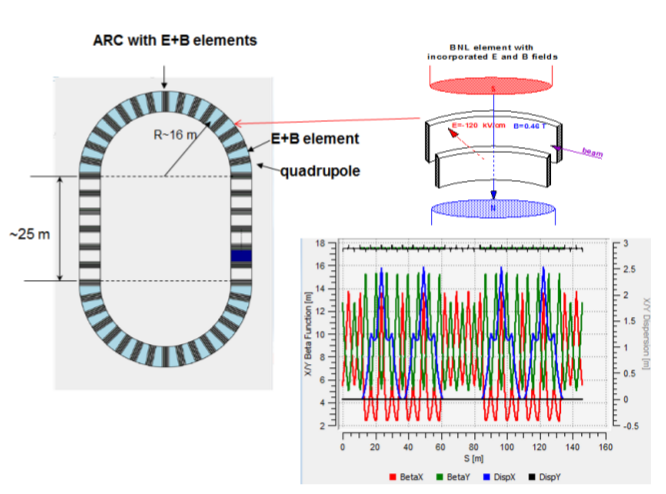
\includegraphics[width=\linewidth]{images/chapter2/BNL_lattice}
	\caption{Вариант кольца, построенного по принципу ``замороженного'' спина. В арках использованы цилиндрические электро-магнитные элементы (Рисунок взят из~\cite{Senichev:Lattices})\label{fig:BNL_lattice}}
\end{figure}

Основная цель FS-концепции кольца --- максимизация ЭДМ сигнала. Однако, следует обратить внимание на то, что строгое выполнение условия замороженности спина возможно только для референсной частицы. Это связано с тем, что, как следует из уравнения~\eqref{eq:TBMT_MDM}, для заданных E-, B-полей, существует уникальное значение Лоренц-фактора $\gamma$, при котором $\W_y^{MDM} = 0$. Таким образом, даже в FS-структуре, спин-векторы большинства частиц ``заморожены'' лишь приблизительно.

\section{Структура с ``квази-замороженным'' спином} \label{sec:QFS_concept}
В QFS-концепции кольца отказываются от непрерывного выполнения условия сонаправленности векторов поляризации и импульса пучка, требуя лишь равенства нулю \emph{совокупного за оборот} угла поворота вектора поляризации относительно импульса в электростатических ($\Phi_s^E$) и магнитных ($\Phi_s^B$) элементах:~\cite{Senichev:Lattices}
\begin{equation*}
	\sum_i \Phi_{s,i}^E = -\sum_j \Phi_{s,j}^B.
\end{equation*}

Как следует из определения спин-тюна (см. раздел~\ref{sec:TBMT_introduction}), угол поворота спин-вектора частицы относительно её импульса в электромагнитном поле $\Phi_s = \nu_s \cdot \Phi$, где $\Phi$ угол поворота импульса, а $\nu_s$ спин-тюн.

Угловая скорость поворота вектора импульса частицы в магнитном поле $\vec B$ есть 
\[
\w_B = \frac qm \frac B \gamma,
\]
в электростатическом $\vec E$:
\[
\w_E = \frac qE \frac{\vec E\times \vec\beta}{c\beta^2\gamma},
\]

из чего следуют выражения для спин-тюна частицы в электростатическом и магнитном полях:
\begin{equation}
	\begin{cases}
		\nu_s^B &= \gamma G, \\
		\nu_s^E &= \beta^2\gamma\bkt{\frac{1}{\gamma^2-1} - G}.
	\end{cases}
\end{equation}

Преимущество кольца QFS-типа над кольцом FS-типа в относительной простоте исполнения: нет необходимости использовать совмещённые цилиндрические электро-магнитные элементы; в двух вариантах QFS-кольца, рассматриваемых ниже, используются 
\begin{enumerate*}[\itshape a\upshape)]
\item либо прямые фильтры Вина, 
\item либо цилиндрические электростатические дефлекторы и магнитные диполи раздельно.
\end{enumerate*}
С другой стороны, из-за появления вертикальной компоненты оси прецессии спина $\bar n_y$, максимальная амплитуда ЭДМ-сигнала уменьшается по сравнению с полностью замороженным случаем. Фактор, на который уменьшается амплитуда~\cite{Senichev:QFS_IPAC15}
\[
J_0(\Phi_s) \approx 1 - \frac{\Phi_s^2}{4},
\]
где $\Phi_s$ есть максимальный угол отклонения горизонтальной проекции вектора спина частицы от вектора импульса. Педположим, что этот угол не превосходит половины \hl{набега спиновой фазы за оборот} $\pi\cdot \gamma G/2n$; в данном контексте $n$ --- периодичность оптики кольца. Поскольку магнитная аномалия дейтрона $G = -0.142$, для рассматриваемых ниже QFS структур $J_0\ge 0.98$.

\subsection{Структура с кодовым названием 6.3}\label{sec:QFS_6_3_lattice}

На Рисунке~\ref{fig:QFS_6_3_lattice} представлена структура, построенная по принципу квази-замороженного спина, в которой электростатические и магнитные поля разделены в пространстве.~\cite{Senichev:Lattices} Электростатические цилиндрические дефлекторы с отрицательной кривизной орбиты используются для компенсации набега фазы, связанного с МДМ-прецессией в магнитных арках.~\cite{Senichev:QFS_IPAC15} Кольцо длины 166.67 м рассчитано на инжекцию пучка дейтронов на энергии 270 МэВ. Для подавления эффектов декогеренции первого порядка используется ВЧ резонатор, с продольным полем $V = 100$ кВ, и рабочей частотой $f_{RF} = 5\cdot f_{rev}$, где $f_{rev} = 0.87$ МГц. Нелинейные эффекты декогеренции подавляются с помощью \hl{шести семейств секступолей}.

\begin{figure}[h!]
	\centering
	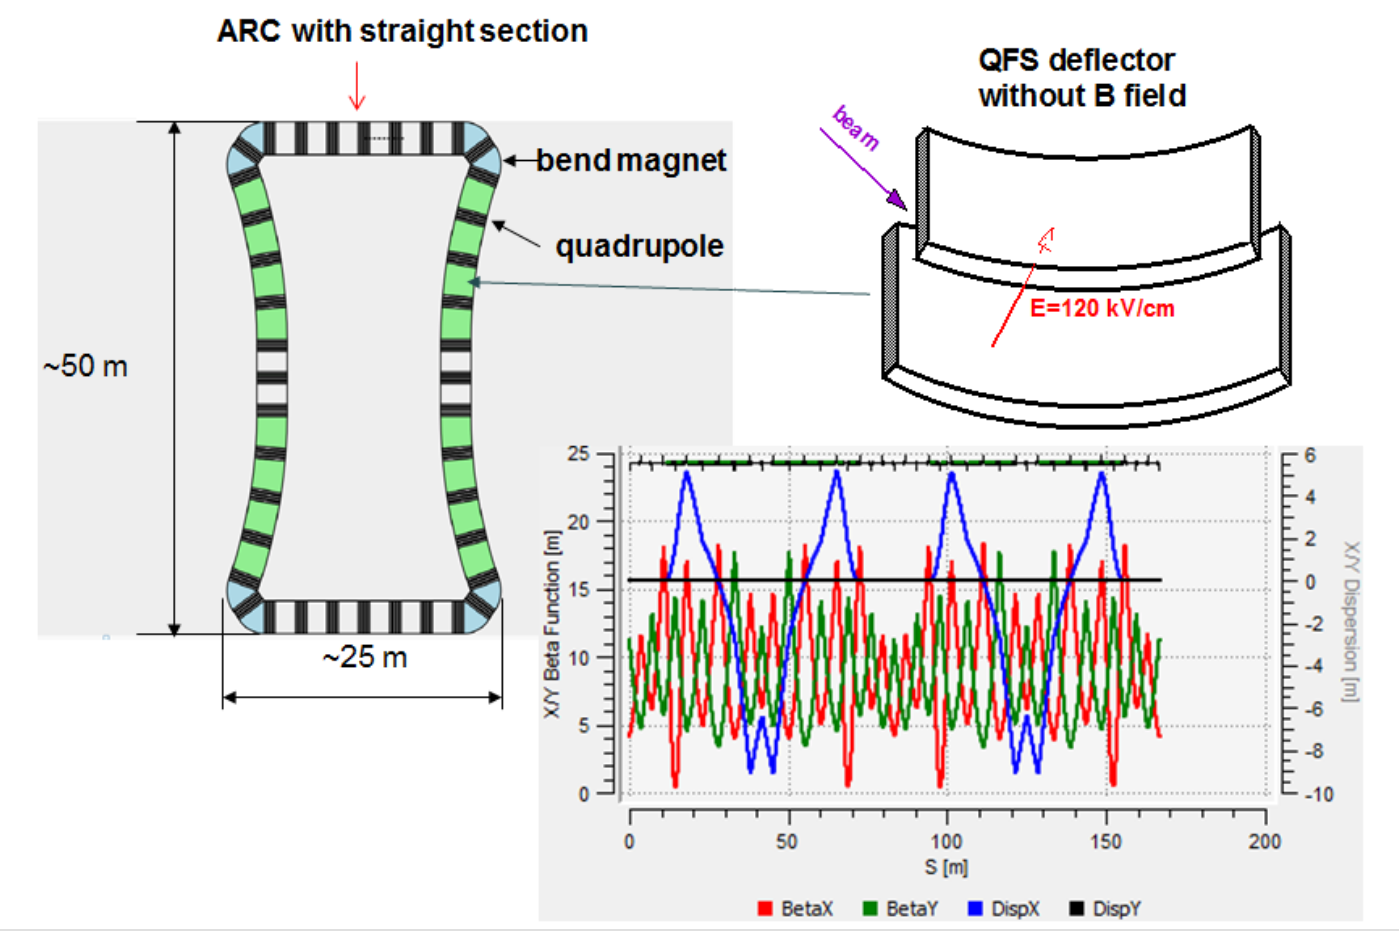
\includegraphics[width=\linewidth]{images/chapter2/6_3_lattice}
	\caption{Вариант кольца, построенного по принципу квази-замороженного спина, дизайн с разделением E- и B-полей. (Рисунок взят из~\cite{Senichev:Lattices})\label{fig:QFS_6_3_lattice}}
\end{figure}

\subsection{Структура с кодовым названием E+B}\label{sec:QFS_EB_lattice}

В структуре, представленной на Рисунке~\ref{fig:QFS_E+B_lattice}, используются прямые, статические фильтры Вина. Это позволяет:
\begin{enumerate*}[\itshape a\upshape)]
	\item исключить нелинейные компоненты электростатического поля, возникающие в связи с кривизной дефлектора, и 
	\item упростить структуру с инженерной точки зрения.
\end{enumerate*}

Длина структуры 149.21 м, энергия инжектируемых дейтронов 270 МэВ. Для подавления эффекта декогеренции первого порядка используется ВЧ-резонатор с продольным напряжением $V = 100$ кВ и частотой $f_{RF} = 5\cdot f_{rev}$, где $f_{rev} = 0.98$ МГц. Нелинейные эффекты декогеренции подавляются с помощью \hl{четырёх семейств секступолей}.
\begin{figure}[h!]
	\centering
	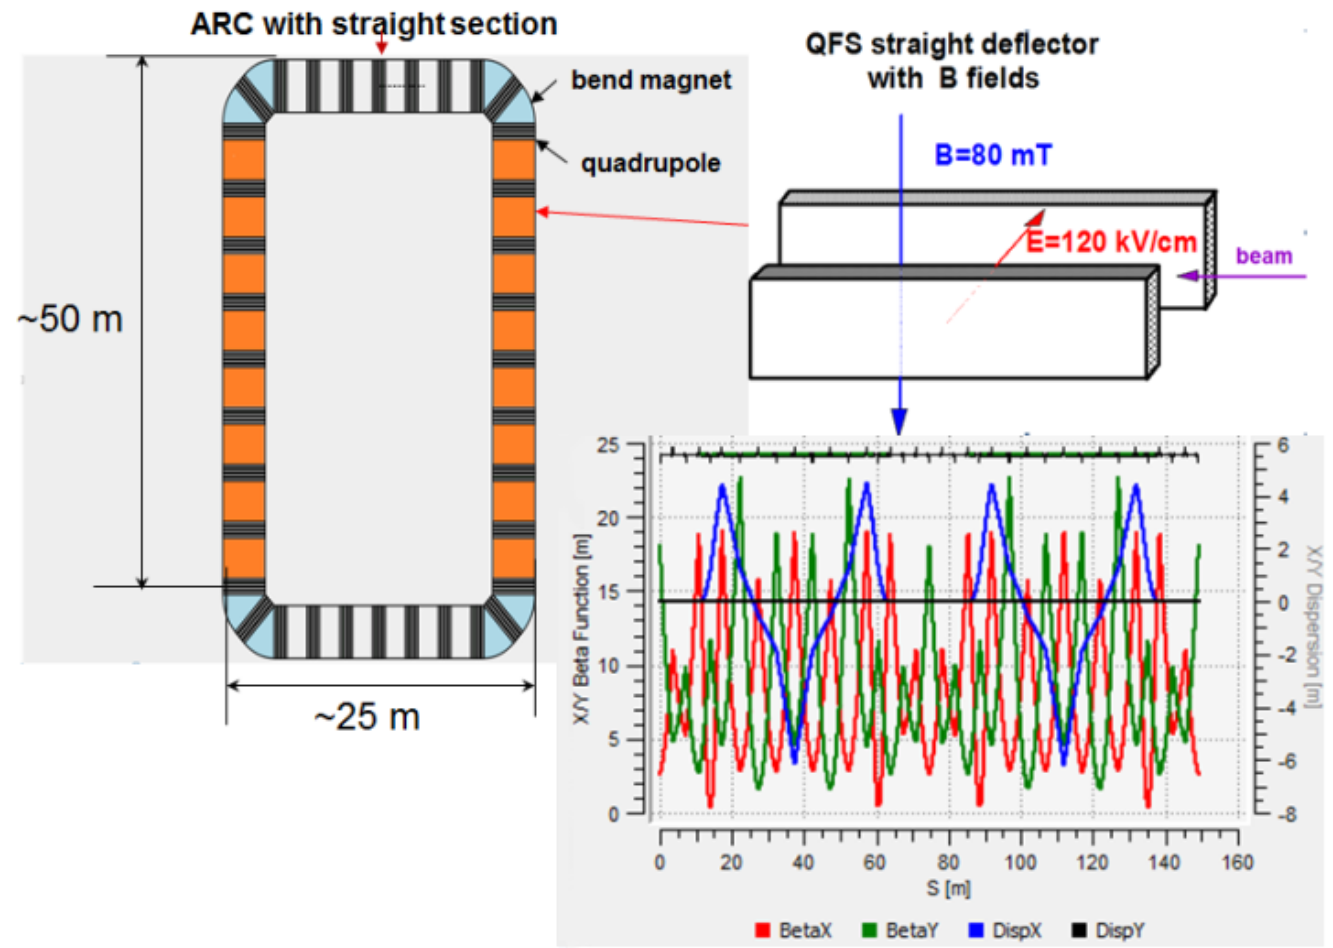
\includegraphics[width=\linewidth]{images/chapter2/E+B_lattice}
	\caption{Вариант кольца, построенного по принципу квази-замороженного спина, дизайн с прямыми фильтрами Вина. (Рисунок взят из~\cite{Senichev:Lattices})\label{fig:QFS_E+B_lattice}}
\end{figure}



           % Глава 2  % moved content to a section of chapter 1
\chapter{Численное моделирование с пмощью кода COSY Infinity} \label{chapt3}

\section{Фальш-сигнал} \label{sect3_1}
Description of how element misalignments were introduced and why so (to preserve the closed orbit). 
Plots: precession frequency vs mean tilt angle
\section{Декогеренция и её оптимизация}
Description of the sextupole strength optimization procedure
Unoptimized vs optimized spin tune plots
\section{Смена полярности ведущего поля} \label{sect3_2}

\clearpage
           % Глава 3
\chapter{Результаты на COSY}\label{chpt4:results-at-COSY}

\section{Ускоритель COSY}


\begin{figure}[h]
	\centering
	\includegraphics[scale=.5]{images/chapter4/800px-COSY_Ring}
	\caption{Синхротрон COSY.\label{fig:COSY_Ring}}
\end{figure}

Синхротрон COSY~\cite{COSY-Ring} --- это уникальная установка, позволяющая проводить эксперименты с
поляризованными и охлаждёнными адронными пучками. До конца 2014 года на нём проводились эксперименты
ANKE, PAX, WASA-at-COSY.~\cite{FZJ:Experiments} Начиная с 2015 года, COSY использовался в качестве
полигона для разработки ускорительных и детекторных технологий, а также подготовки и проведения
прецезионных экспериментов с поляризованными пучками: TRIC (Time Reversal Invariance at Cosy) и
JEDI (J\"ulich Electric Dipole moment Investigations).

Для инжекции ионов $H^-$ и $D^-$ в COSY  используется циклотрон JULIC (J\"ulich Light Ion Cyclotron), предоставляющий 8 мкА неполяризованных (или 1 мкА поляризованных) ионов $H^-$ с импульсом 45 МэВ/с. При инжекции отрицательные ионы проходят через углеродный стриппер для изменения их заряда на положительный. Экстракция пучка из циклотрона производится с помощью септум-дефлектора.~\cite{JULIC-Injector}

Возможности направляющей магнитной системы синхротрона ограничивают импульс пучка в диапазоне до 3700 МэВ/с. Экстракция из кольца осуществляется с помощью кикера.

На COSY доступны два типа охлаждения пучка: электронное (диапазон энергий электронов в ``старом'' и ``новом'' кулере -- 20-100 кэВ и 20 кэВ - 2 МэВ, соответственно) и стохастическое. 
%
Два электронных кулера, установленые в кольце на прямой секции, обеспечивают электронное охлаждение во всём диапазоне энергий кольца. Система стохастического охлаждения обеспечивает охлаждение пучка при импульсах 1.5-3.7 ГэВ/с.

Поляризация пучка непрерывно отслеживается на поляриметре  EDDA. Также недавно был установлен поляриметр на основе детекторов WASA, а в конце 2019 года будет установлен новый поляриметр на основе LYSO-сцинцилляторов.
Поляризация протонов достигает 75\% вплоть до наивысших значений импульса; векторная и тензорная поляризации дейтронного пучка достигают 60\%.


\section{Спин-тюн мэппинг}\label{sec:COSY:spin-tune-mapping}
\newcommand{\cbar}{\vec c}
\newcommand{\wbar}{\vec w}

Хотя это напрямую не связано с детектированием ЭДМ частицы методом замороженного спина,
измерение частоты прецессии поляризации пучка вокруг направления ведущего поля ускорителя
является важным шагом к пониманию и контролю спин-прецессии в накопительном кольце.

\subsection{Возможные наблюдаемые}
В идеальном магнитном накопительном кольце, спины частиц пучка прецессируют вокруг ведущего магнитного
поля. Введём правостороннюю систему координат, связанную с центром масс пучка, так что орт $\hat y$ будет
сонаправлен с ведущим полем, $\hat z$ сонаправлен с импульсом референсной частицы. ЭДМ влияет
на спиновую динамику пучка двумя путями. Во-первых, он отклоняет ось стабильного спина референсной частицы
от строго вертикального направления:~\cite{COSY:SpinTuneMapping}
\[
\cbar = \hat x\sin\xi_{EDM} + \hat y\cos\xi_{EDM}, ~~ \tan\xi_{EDM} = \frac{\eta\beta}{G}.
\]

Во-вторых, он изменяет значение спин-тюна, от его канонического $\nu_s = \gamma G$ на
\[
\nu_s = \frac{\gamma G}{\cos\xi_{EDM}}.
\]

На COSY используется резонансный метод измерения спин-тюна, основанный на применении
ВЧ Вин-фильтра (ВЧ ВФ).~\cite{COSY:Partially-Frozen-Spin} ВЧ ВФ с вертикально-направленным магнитным,
радиально-направленным электрическим полем, создаёт ВЧ-модулируемую МДМ прецессию поляризации пучка
вокруг вертикальной оси. При этом, если частота ВЧ поля
фильтра совпадает с частотой прецессии спина без него, модуляция спин-тюна резонирует с ЭДМ взаимодействием
с электрическим полем $\vec E \propto \vec\beta\times\vec B$, и генерирует прецессию спина вокруг радиальной оси.

Сила резонанса
\[
\epsilon = \frac12 \chi_{WF}|\cbar\times\wbar|,
\]
где $\cbar$ обозначает ось стабильного спина кольца в месте расположения ВЧ ВФ \emph{до} его включения,
а $\chi_{WF}$ и $\wbar$ --- угол поворота спина и направление магнитного поля в ВЧ ВФ.

В идеальном ВЧ ВФ
\[
\epsilon = \frac12 \chi_{WF}\sin\xi_{EDM},
\]
равна нулю, если ЭДМ $d$, а значит и $\xi_{EDM}$, равны нулю.~\cite[стр.~5]{COSY:SpinTuneMapping}

Гораздо более выгодным было бы измерение направления самой оси стабильно спина в ускорителе, а не силы резонанса,
поскольку последняя аттенюирована фактором $\chi_{WF}\ll 1$. Проблема заключается в том, что, как и ЭДМ,
неидеальности ускорителя дают вклад в наклон оси от вертикального направления. В связи с этим, задача анализа
неидеальности накопительного кольца стала приоритетной в исследованиях на COSY.

\subsection{Наблюдение наклона оси стабильного спина}
Поскольку спин-тюн является очень точной наблюдаемой, которая к тому же чувствительна к неидеальностям
в ускорителе, она может быть использована для определения направления оси стабильного спина $\cbar$.
Для этого используются два соленоида, которые выступают в качестве искусственных неидеальностей. Обозначив
угол поворота спина в соленоиде $\chi_{AI}$, направление его магнитного поля $\vec k$,


\subsection{Процедура измерения и анализа}
Одной из задач эксперимента, проведённого в 2014 году на COSY было изучение оси стабильного спина, путём
введения искусственных неидеальностей


\subsection{Результаты}


\section{Оптимизация времени когерентности}
\newcommand{\dpop}{\Delta p/p}

Изначальной целью экспериментов по изучению времени когерентности спина (Spin Coherence Time) на COSY было подтверждение возможности секступольных полей противодействовать дисперсии спин-тюнов, ассоциированной с 
эмиттансом и дисперсией импульсов ($\dpop$) частиц пучка.~\cite{COSY:SCT:IPAC15} На настоящий момент, оптимизация SCT является первой фазой любого предварительного эксперимента по поиску ЭДМ на COSY.

Секступольное подавление декогеренции используется совместно с электронным охлаждением пучка, для
уменьшения его фазового объёма, и банчингом, для подавления линейного вклада дисперсии импульсов частиц 
в декогеренцию. Секступоли, располагающиеся в арках, призваны подавлять эффект декогеренции второго порядка.

Для контроля декогеренции используются три семейства секступолей, которые маркированны соответственно: MXG, расположенный в максимуме дисперсионной функции, и контролирующий эффект декогеренции связанный с $\dpop$; MXS, расположенный в максимуме горизонтальной бета-функции $\beta_x$, и контролирующий дисперсию, связанную с горизонтальными бетатронными колебаниями; MXL, в максимуме $\beta_y$, контролирующий дисперсию, возникающую из-за вертикальных бетатронных колебаний.

\begin{figure}[H]\centering
	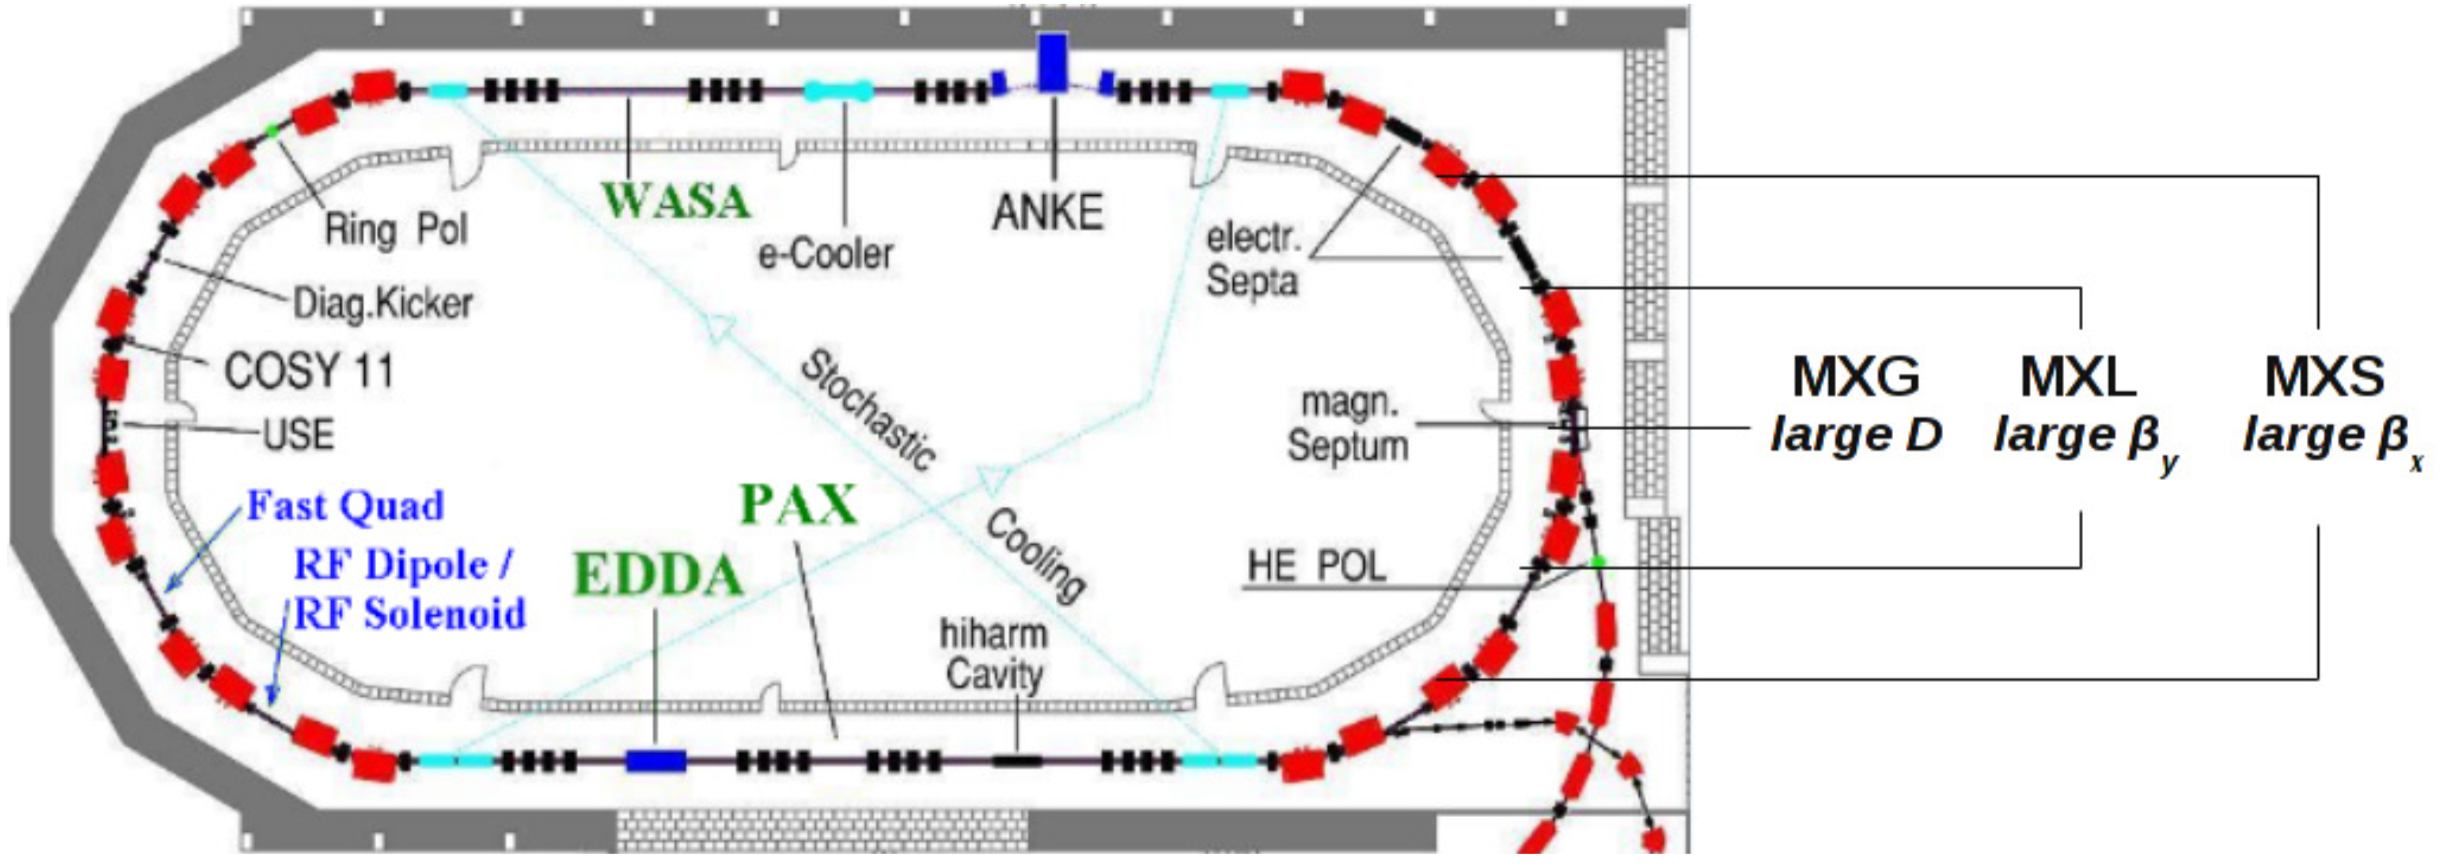
\includegraphics[width=\linewidth]{images/chapter4/COSY-sextupoles}
	\caption{Кольцо COSY с отмеченными положениями секступолей для контроля времени когерентности спина. (Рисунок взят из~\cite{Guidoboni:STORI14})}
\end{figure}

\subsection{Процедура оптимизации}
В этом разделе описана процедура оптимизации SCT, на примере эксперимента 2014 года.~\cite{Guidoboni:STORI14} Первый оптимизационный эксперимент проводился в 2012 году, но тогда варьировалась только напряжённость поля секступоля MXS. В 2014 году впервые проведён полноценный (варьировались градиенты всех трёх секступолей) эксперимент по оптимизации SCT. 

Чтобы отделить эффекты декогеренции, связанные с конечностью эмиттанса пучка, и с вторым порядком дисперсии импульсов частиц $(\dpop)^2$, подготовка пучка к эксперименту проводится по-разному.

Для получения пучка с большим разбросом $(\dpop)^2$, поляризованный дейтронный пучок с импульсом $p=0.97$~ГэВ/с сначала охлаждается в течении 60 секунд для минимизации его эмиттанса. После отключения охлаждения пучок банчируется (гармоническое число $h=1$). Банчирование необходимо для подавления линейных эффектов декогеренции.

В случае изучения декогеренции, связанной с горизонтальным эмиттансом пучка,~\footnote{Декогеренция, связанная с вертикальным эмиттансом не может быть изучена ввиду ограничений по аксептансу.} охлаждение и банчирование проводятся одновременно в течении первых 60 секунд, после чего охлаждение отключается, и на пять секунд включается горизонтальное нагревание. Пучок нагревается подачей белого шума на обкладки конденсатора горизонтального кикера.

В обоих случаях, пучок инжектируется с вертикально-ориентированным вектором поляризации. Поворот поляризации в горизонтальную плоскость производится ВЧ соленоидом, после подготовки пучка, на 80-й секунде.

Мониторинг поляризации пучка производится непрерывно, путём приложения белого шума на вертикальный кикер, для экстракции пучка на 17-мм углеродную мишень. Далее, эластично-рассеянные дейтроны детектируются на поляриметре EDDA. Эластичное рассеяние дейтронов на углеродной мишени чувствительно к направлению спина, и имеет большое сечение взаимодействия. 

Сцинтилляторы поляриметра поделены на четыре группы: верхние, нижние, левые, правые; асимметрия частот событий на левом и правом детекторах пропорциональна вертикальной поляризации, а на верхнем и нижнем --- горизонтальной поляризации. Прецессия поляризации пучка в горизонтальной плоскости происходит с частотой, значительно превышающей частоту выборки поляриметра, поэтому в 2012 году была разработана специальная система сбора данных~\cite{COSY:DAQ}.

По результатам эксперимента~\cite{Guidoboni:STORI14} была доказана возможность получать на COSY SCT 
свыше 1~000~секунд. 

\subsection{Изменение SCT при переходе от внешней к внутренней части пучка}
Ниже представлены результаты оптимизации SCT, полученные в период измерений апрель-май 2019 года. 

На серии рисунков~\ref{fig:April2019:Polarization} представлены измерения асимметрии частоты событий на верхнем и нижнем детекторах (так называемая асимметрия верх-низ), которая пропорциональна горизонтальной компоненте поляризации пучка. На первых двух рисунках можно наблюдать, что на начальном этапе (в промежутке от 100 до 150 секунд) деполяризация происходит со значительной скоростью, но во второй половине цикла скорость деполяризации падает. На Рисунке~\ref{fig:Polariation:recovery-from-halo-to-core} особенно, мы видим, что в промежутке времени приблизительно от 130 до 150 секунд поляризация начинает возрастать, прежде чем снова спадает со значительно меньшей скоростью.
\begin{figure}[H]\centering
	\subbottom[SCT = $20.87 \pm 1.49$ секунд\label{fig:Polariation:recovery-from-halo-to-core}]{%
		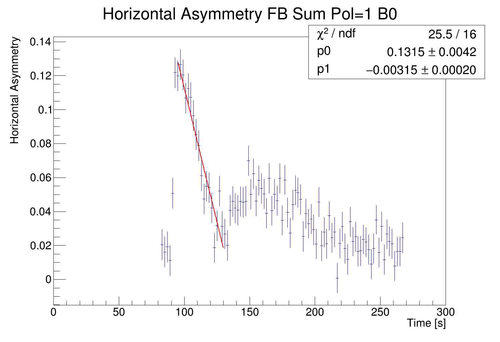
\includegraphics[height=.35\paperheight]{images/chapter4/SCT-April-2019/11th_19-55}}
\end{figure}
\begin{figure}[H]\centering
	\contsubbottom[SCT = $42.3 \pm 2.2$ секунд]{%
		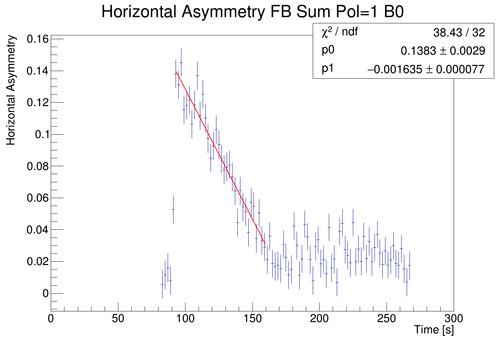
\includegraphics[height=.35\paperheight]{images/chapter4/SCT-April-2019/11th_20-20}}
\end{figure}
\begin{figure}[H]\centering
	\contsubbottom[SCT = $70.6 \pm 4.1$ секунд\label{fig:Polarization:halo-and-core-similar}]{%
		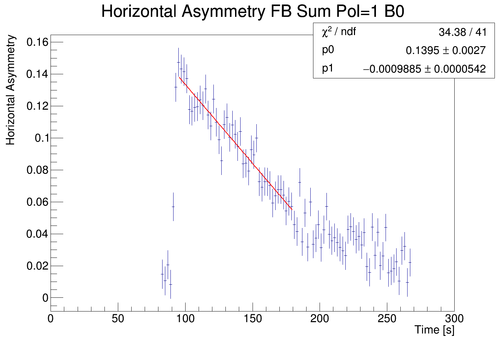
\includegraphics[height=.35\paperheight]{images/chapter4/SCT-April-2019/11th_20-31}}
\end{figure}
\begin{figure}[H]\centering
	\contsubbottom[SCT = $302.0 \pm 27.5$ секунд]{%
		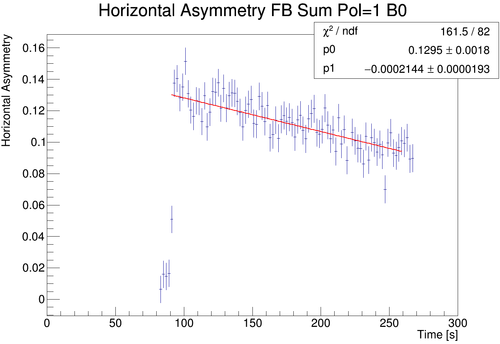
\includegraphics[height=.35\paperheight]{images/chapter4/SCT-April-2019/13th_03-23}}
	\caption{Измерения горизонтальной поляризации во время оптимизации времени когерентности спина при подготовке к эксперименту по поиску аксионов в апреле 2019 года\label{fig:April2019:Polarization}}
\end{figure}

Такое поведение поляризации на данный момент объясняется неоднородностью поляризованности пучка. В первой половине цикла на детектор преимущественно попадают частицы из внешней (halo) части пучка (оболочки); к второй половине цикла начинается выборка частиц из центральной (core) части (ядра). Поскольку ядро плотнее чем оболочка, разброс длин орбит частиц ядра меньше, чем частиц оболочки, а значит меньше и разброс спин тюнов частиц.

\subsection{Зависимость времени когерентности спина от силы секступоля}
На Рисунках~\ref{fig:SCT_scan} представлена зависимость времени когерентности спина от относительной силы поля, соответственно MXL и MXG секступолей, измеренная во время оптимизации в апреле 2019 года. Наблюдается зависимость резонансного типа времени когерентности от значений относительной силы поля секступолей.

\begin{figure}[H]\centering
	\subbottom[Секступоль MXL]{%
		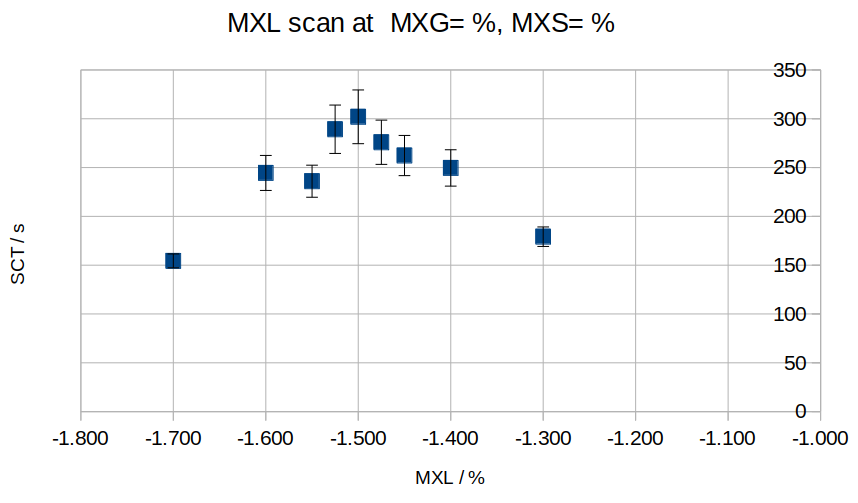
\includegraphics[height=.3\paperheight]{images/chapter4/SCT-April-2019/MXL_scan}}
\end{figure}
\begin{figure}[H]\centering
	\contsubbottom[Секступоль MXG]{%
		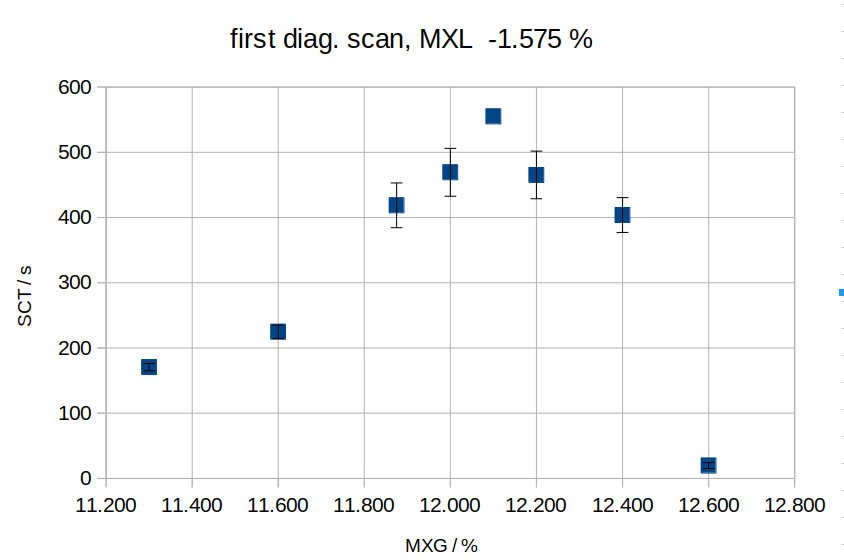
\includegraphics[height=.3\paperheight]{images/chapter4/SCT-April-2019/MXG_scan}
	}
	\caption{Зависимость SCT от градиента секступоля\label{fig:SCT_scan}}
\end{figure}

Мы проверили, соблюдается ли такая же зависимость в рамках нашей численной модели, с учётом того, что измерения на COSY проводятся на энергии, значительно удалённой от спин-резонансной. На Рисунке~\ref{fig:SCT_resonance} изображена зависимость стандартного отклонения спин-тюнов частиц пучка от значения градиента подавляющего декогеренцию секступоля (данные взяты из симуляции, описанной в разделе~\ref{sec:decoh:sim-imperfect}). Зависимость показывает такой же резонансный характер, как и данные эксперимента.

\begin{figure}[H]
	\centering
	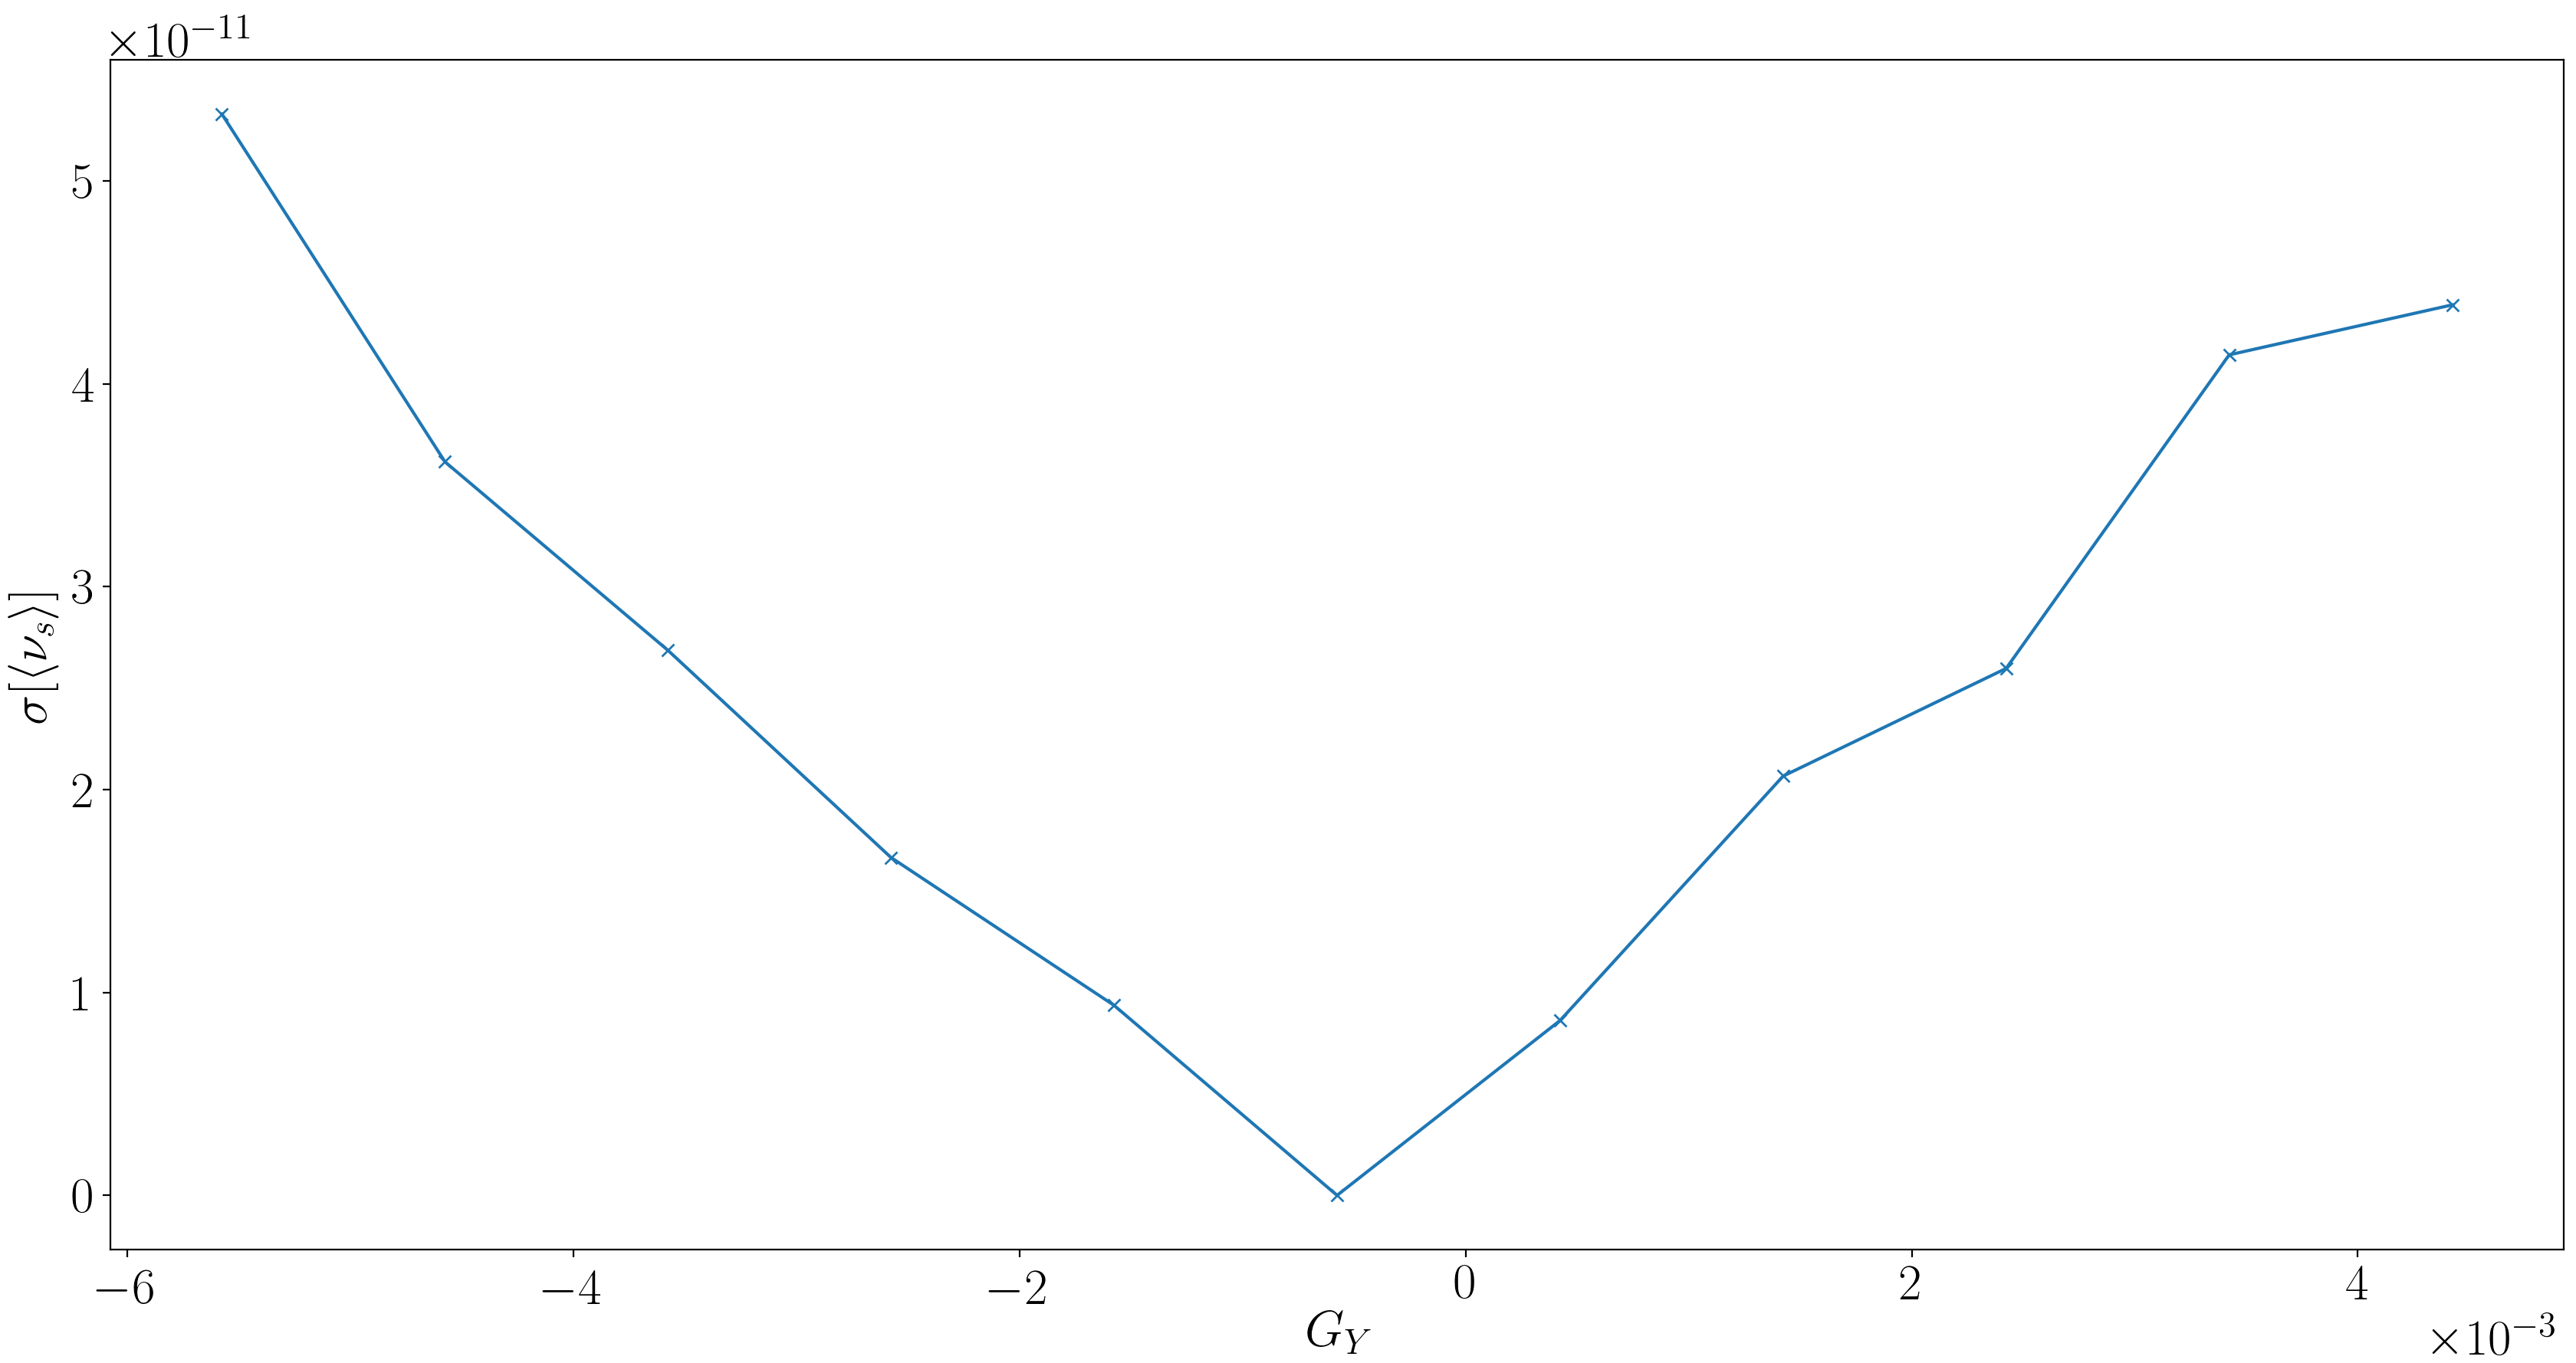
\includegraphics[width=\linewidth]{images/decoh_sim/stune_sd_vs_sext_strength_resonance}
	\caption{Зависимость стандартного отклонения спин-тюнов частиц банча от используемого градиента подавляющего декогеренцию секступоля.\label{fig:SCT_resonance}}
\end{figure}



\clearpage
		   % Глава 4
\chapter*{Заключение}                       % Заголовок
\addcontentsline{toc}{chapter}{Заключение}  % Добавляем его в оглавление

%% Согласно ГОСТ Р 7.0.11-2011:
%% 5.3.3 В заключении диссертации излагают итоги выполненного исследования, рекомендации, перспективы дальнейшей разработки темы.
%% 9.2.3 В заключении автореферата диссертации излагают итоги данного исследования, рекомендации и перспективы дальнейшей разработки темы.
%% Поэтому имеет смысл сделать эту часть общей и загрузить из одного файла в автореферат и в диссертацию:

Основные результаты работы заключаются в следующем.
%% Согласно ГОСТ Р 7.0.11-2011:
%% 5.3.3 В заключении диссертации излагают итоги выполненного исследования, рекомендации, перспективы дальнейшей разработки темы.
%% 9.2.3 В заключении автореферата диссертации излагают итоги данного исследования, рекомендации и перспективы дальнейшей разработки темы.

\begin{enumerate}
	\item Разработан метод измерения электрического дипольного момента дейтрона, 
	основанный исключительно на измерении частоты прецессии спина.
	\item Предложен принцип построения магнитооптической структуры кольца-накопителя, 
	ориентированного на поиск электрического дипольного момента дейтрона.
	\item Получены результаты исследования спин-декогеренции пучка дейтронов в окрестности 
	состояния ``замороженного спина'', а также метод подавления спин-декогеренции, основанный на использовании нелинейных элементов.
	\item Исследованы эффекты различного рода несовершенств элементов накопительного кольца 
	на спин-орбитальную динамику пучка.
	\item Проведено численное моделирование матода калибровки нормализованной частоты прецессии спина 
	при попеременной смене полярности ведущего поля накопительного кольца.
	\item Исследованы систематические ошибки в различных предложениях по проведению эксперимента 
	по поиску электрического дипольного момента; проведён сравнительный анализ этих предлодений 
	с методом Frequency Domain.
	\item Проведена оценка статистических свойств Frequency Domain метода измерения 
	электрического дипольного момента в накопительном кольце.
\end{enumerate}
%\begin{enumerate}
%  \item Были изучены эффекты спиновой динамики, составляющие систематические ошибки эксперимента по поиску
%  электрического дипольного момента частицы методом замороженного спина в накопительном кольце, как то:
%  \begin{itemize}
%  	\item возмущения спиновой динамики вызванные бетатронным движением частицы;
%  	\item декогеренция спинов частиц пучка;
%  	\item МДМ прецессия спина, вызванная неидеальностями ускорителя.
%  \end{itemize}
%  \item Для каждого из эффектов, было описано средство борьбы, и проведено численное моделирование,
%  подтверждающее его эффективность.
%  \item Были сформулированы:
%  \begin{itemize}
%  	\item понятия методов пространственной и временной областей;
%  	\item понятие двумерно-замороженного спина;
%  	\item необходимые условия успешного измерения ЭДМ в накопительном кольце;
%  	\item метод Frequency Domain, удовлетворяющий всем сформулированным условиям.
%  \end{itemize}
%  \item Описаны структуры накопительных колец с непрерывно- и квази-замороженным спином.
%\end{enumerate}


В заключение, автор выражает благодарность научным руководителям, Сеничеву~Ю.~В. и Полозову~С.~М., за научное руководство, Салееву~А.~В. и Валетову~Е.~В. за плодотворные дискуссии, Институту Ядерных Исследований (IKP-2) Исследовательского центра ``Юлих,'' и в частности коллективу коллаборации JEDI, за возможность участвовать в проекте по поиску ЭДМ.
      % Заключение
%\include{Dissertation/acronyms}        % Список сокращений и условных обозначений
%\include{Dissertation/dictionary}      % Словарь терминов
\include{Dissertation/references}      % Список литературы
\include{Dissertation/lists}           % Списки таблиц и изображений (иллюстративный материал)

%%% Настройки для приложений
\appendix
% Оформление заголовков приложений ближе к ГОСТ:
\setlength{\midchapskip}{20pt}
\renewcommand*{\afterchapternum}{\par\nobreak\vskip \midchapskip}
\renewcommand\thechapter{\Asbuk{chapter}} % Чтобы приложения русскими буквами нумеровались

%\include{Dissertation/appendix}        % Приложения
\chapter{Статистический анализ}\label{Apx:Stats}
\newcommand{\cnt}{c}
\newcommand{\meas}{\epsilon}
\newcommand{\dt}{\Delta t}
\newcommand{\dtm}{\dt_{\meas}}
\newcommand{\dtc}{\dt_{\cnt}}
\newcommand{\Ncm}{{n_{\sfrac{\cnt}{\meas}}}}
\newcommand{\Nmnd}{{n_{\sfrac{\meas}{zc}}}}
\newcommand{\Nnd}{{n_{zc}}}
\newcommand{\Nm}{{n_{\meas}}}
\newcommand{\Ncnt}{{n_{\cnt}}}
\newcommand{\LTb}{\tau_b}
\newcommand{\LTd}{\tau_d}
\newcommand{\lamb}{\lambda_b}
\newcommand{\lamd}{\lambda_d}

\DeclareDocumentCommand{\mupp}{s}{\mu'_\phi\IfBooleanTF{#1}{}{(t_i)}}
\DeclareDocumentCommand{\mudpp}{s}{\mu''_{\phi^2}\IfBooleanTF{#1}{}{(t_i)}}
\newcommand{\pars}{\boldsymbol{\theta}}
\DeclareDocumentCommand{\XpctO}{m}{\Xpct{#1}[\pars_0]}
\DeclareDocumentCommand{\var}{O{}mo}{\mathrm{var}_{#1}\bkt*{#2\IfValueT{#3}{\vert~ #3}}}
\DeclareDocumentCommand{\Fisher}{O{}D(){\pars_0}}{I_{#1}(#2)}
\newcommand{\y}{\mathbf{y}}

\usepgfplotslibrary{fillbetween}

\chapter{Статистическое моделирование}\label{Apx:Stats}
В этой главе мы рассматриваем стандартную ошибку оценки частоты прецессии спина, 
в эксперименте по поиску ЭДМ дейтрона в накопительном кольце. 
Основное рассмотрение начинается с раздела~\ref{Apx:Stats:Detector_counting_rate}; 
раздел~\ref{Apx:Stats:Prelim} предоставляет обоснование некоторым используемым понятиям 
(таким как информация Фишера выборки, информативность точки), но может быть пропущен.

Частота прецессии спина определяется путём фитирования данных поляриметрии синусоидальной функцией
 ${f(t) = a\cdot\sin(\w\cdot t + \delta)}$ с постоянными параметрами $(a,\w,\delta)$. 
 Данные о поляризации получают при рассеянии пучка на углеродной мишени. 
 Двумя важными обстоятельствами поляриметрии являются:
\begin{enumerate*}[(1)]
	\item уменьшение числа частиц в пучке при каждом измерении поляризации, и
	\item деполяризация.
\end{enumerate*}

В связи с первым обстоятельством возникает желание использовать каждое измерение поляризации 
максимально эффективно. В выборке измеренний сигнала, максимальной информативностью обладают точки,
измеренные в моменты, когда сигнал имел наибольшую скорость изменения 
(см. раздел~\ref{Apx:Stats:Prelim} ниже). По этой причине возникла идея измерять поляризацию пучка 
только в моменты пересечения ею нуля (модулированная схема измерения): 
таким образом увеличивается время жизни пучка, а потеря частиц происходит наиболее выгодным образом. 

При этом необходимо отметить, что анализирующая способность детектора как раз максимальна в экстремумах, 
и стремится к нулю в узлах сигнала. Это ограничивает возможность увеличения эффективности выборки
модулированной схемой: наиболее ценные для нас измерения поляризации имеют наименьшую точность, 
а наименее ценные --- максимальную. В связи с этим, мы пришли к выводу о нецелесообразности использования
модулированной схеме выборки.

Также, это влияет и на гетероскедастичность данных: в  проведённой нами симуляции 
мы использовали непериодическую модель роста ошибки стандартного отклонения 
измерения поляризации из~\cite[стр.~18]{Eversmann:Thesis}, в то время как 
колебания анализирующей способности детектора вводят периодическую зависимость от времени.

Фактор деполяризации в свою очередь ограничивает наши возможности по продлению времени жизни пучка, 
а следовательно накладывает ограничения и на длительность измерительного цикла, 
возможную точность единичной оценки частоты спин-прецессии, 
и длительность полного времени измерения ЭДМ.

В следующих разделах мы рассмотрим модель временн\'{о}й зависимости частоты событий на детекторе, 
введём понятие асимметрии сечения взаимодействия, и определим адекватную, ввиду деполяризации,
длительность измерительного цикла. Также, мы промоделируем статистическую обработку данных, и 
попытаемся определить потенциал применения модулированной схемы измерения поляризации.

\section{Предварительный анализ}\label{Apx:Stats:Prelim}

Вероятность наблюдения величины ${y_i = y(t_i)}$, при ожидании $\mu(t_i)$ и нормальном распределении ошибки:
\begin{align*}
f(y_i|\pars) &= \frac{1}{\sqrt{2\pi\nu}}\exp\bkt{-\frac12\frac{(y_i - \mu(t_i))^2}{\nu}}, \\
\pars 		  &= (\nu,\w,\phi),\\
\mu(t_i) 	  &= N_0\bkt{1 + P\sin(\w t_i + \phi)}.
\end{align*}

Вероятность наблюдения набора измерений $\y = (y_1,\dots, y_K)$, предполагая что они все происходят из одного и того же распределения, это произведение вероятностей, взятое как функция параметров:
\begin{align*}
\mathcal{L}(\pars|\y) &= \prod_i f(y_i|\pars);
\shortintertext{логарифм вероятности}
\ell(\pars|\y) &= -\frac{K}{2}\log2\pi - \frac{K}{2}\log\nu - \frac{1}{2\nu}\sum_i\epsilon_i^2,
~ \epsilon_i = y_i- \mu(t_i).
\end{align*}
Обычными предположениями на ошибку измерений являются равенство нулю её ожидания, и строгая экзогенность:
\[
\XpctO{\epsilon_i} = \XpctO{t_i\epsilon_i} = 0.
\]

В нашем случае, связь между производными ождидания:
\begin{align*}
\mu'_\phi	&= N_0P\cos(\w t + \phi), \\
\mu'_\w &= t\cdot\mu'_\phi, \epsilon'_\xi = -\mu'_\xi.
\end{align*}

%% Производные логарифма вероятности:
%% \begin{align*}
%% \ell'_\nu 		&= -\frac{K}{2\nu} + \frac{1}{2\nu^2}\sum_i\epsilon_i^2;  & \\
%% \ell'_\w 	&= \frac1\nu\sum_i\mupp t_i\epsilon_i;  & \\
%% \ell'_\phi		&= \frac1\nu \sum_i \mupp\epsilon_i; & \\
%% %
%% \ell''_{\nu^2}		&= \frac{K}{2\nu^2} - \frac{1}{\nu^3}\sum_i\epsilon_i^2, 
%% 	&-\XpctO{\ell''_{\nu^2}} = \frac{K}{2\nu^2} - \frac{1}{\nu^3}\sum_i\nu = \frac{K}{2\nu^2};\\
%% \ell''_{\nu\w}	&= -\frac{1}{\nu^2}\sum_i\mupp t_i\epsilon_i, 
%% 	&-\XpctO{\ell''_{\nu\w}} = \frac{1}{\nu^2}\sum_i\mupp\XpctO{t_i\epsilon_i} = 0;\\
%% \ell''_{\nu\phi}	&= -\frac{1}{\nu^2}\sum_i\mupp \epsilon_i, 
%% 	&-\XpctO{\ell''_{\nu\phi}} = \frac{1}{\nu^2}\sum_i\mupp\XpctO{\epsilon_i} = 0; \\
%% \ell''_{\phi^2}		&= \frac1\nu\sum_i\bkt{\mudpp \epsilon_i - \bkt{\mupp}^2}, 
%% 	&-\XpctO{\ell''_{\phi^2}} = \frac1\nu\sum_i\bkt{\bkt{\mupp}^2 - \mudpp\XpctO{\epsilon_i}} = \frac1\nu\sum_i\bkt{\mupp}^2;\\
%% \ell''_{\phi\w}	&= \frac1\nu\sum_i\bkt{\mudpp t_i\epsilon_i - \bkt{\mupp}^2t_i}, 
%% 	&-\XpctO{\ell''_{\phi\w}} = \frac1\nu\sum_i\bkt{t_i\bkt{\mupp}^2 - \mudpp\XpctO{t_i\epsilon_i}} = \frac1\nu\sum_i t_i\bkt{\mupp}^2;\\
%% \ell''_{\w^2}	&= \frac1\nu\sum_i\bkt{\mudpp t_i^2\epsilon_i - \bkt{\mupp t_i}^2},
%% 	& -\XpctO{\ell''_{\w^2}} = \frac1\nu\sum_i\bkt{\bkt{t_i\mupp}^2 - \mudpp\XpctO{t_i^2\epsilon_i}} = \frac1\nu\sum_i\bkt{t_i\mupp}^2.
%% \end{align*}

\subsection{Дисперсия оценки частоты}
После вычисления производных логарифма вероятности (и их ожиданий), получим матрицу Фишера: 
\[
\Fisher = \begin{pmatrix}
\sfrac{K}{2\nu} & 0 								& 0 \\
0 				& \sfrac1\nu\sum\bkt{t_i\mupp}^2	& \sfrac1\nu\sum t_i\bkt{\mupp}^2 \\
0				& \sfrac1\nu\sum t_i\bkt{\mupp}^2	&\sfrac1\nu\sum\bkt{\mupp}^2
\end{pmatrix}.
\]
Определитель матрицы
\newcommand{\STM}{\alpha}
\[
|\Fisher| = \frac{K}{2\nu^3}\underbrace{\bkt{\sum\bkt{t_i\mupp}^2\sum\bkt{\mupp}^2 - \bkt{\sum t_i\bkt{\mupp}^2}^2}}_{\STM}.
\]
Ковариационная матрица
\[
vcov = \begin{pmatrix}
\sfrac{2\nu}{K}& 0									& 0				\\
0				&\nu\frac{\sum\bkt{\mupp}^2}{\STM}		&\nu\frac{\sum t_i\bkt{\mupp}^2}{\STM}\\
0				&\nu\frac{\sum t_i\bkt{\mupp}^2}{\STM}	&\nu\frac{\sum\bkt{t_i\mupp}^2}{\STM}
\end{pmatrix}.
\]

Дисперсия оценки частоты
\begin{equation}\label{eq:Var1}
\var{\hat{\w}} = \nu\frac{\sum\bkt{\mupp}^2}{\sum\bkt{t_i\mupp}^2\sum\bkt{\mupp}^2 - \bkt{\sum t_i\bkt{\mupp}^2}^2}.
\end{equation}

\paragraph{Проверка.} Положим ${\mu(t_i) = \phi + \w t_i}$. 

В этом случае ${\mupp = 1}$, 
${\mu'_\w(t_i) = t_i = t_i\cdot\mupp}$, и определитель матрицы Фишера упрощается:
\begin{align*}
|\Fisher| &= \frac{K}{2\nu^4}\bkt{K\sum_i t_i^2 - \bkt{\sum t_i}^2} \\
&= \frac{K^3}{2\nu^4}\bkt{\frac1K\sum t_i^2 - \avg{t}^2} \\
&= \frac{K}{2\nu^4}\cdot\underbrace{K\sum\bkt{t_i - \avg{t}}^2}_{\STM},
\end{align*}
\newcommand{\SSX}{\sum\bkt{t_i - \avg{t}}^2}
а ковариационная матрица становится
\[
vcov = \begin{pmatrix}
2\sfrac{\nu^2}{K}& 0									& 0				\\
0				&\frac{\nu}{\SSX}		&\nu\frac{\sum t_i}{K\SSX}\\
0				&\nu\frac{\sum t_i}{K\SSX}	&\nu\frac{\sum t_i^2}{K\SSX}
\end{pmatrix},
\]
с хорошо известным выражением дисперсии оценки наклона прямой
\[
\var{\hat\w} = \frac{\nu}{\SSX}.
\]

Обозначим ${\bkt{\mupp}^2 = (N_0P)^2\cos^2(\w t_i + \phi) \equiv x_i}$. 
Уравнение~\eqref{eq:Var1} может быть записано в виде:
\begin{align}
\var{\hat\w} &= \frac{\nu}{\sum_j x_j \bkt{\sum_i t_i^2 \frac{x_i}{\sum_j x_j} - \bkt{\sum_i t_i \frac{x_i}{\sum_j x_j}}^2}} \notag\\
&= \frac{\nu}{\sum_j x_j \sum_i w_i\bkt{t_i - \avg{t}[w]}^2} \notag\\
&= \frac{\nu}{\sum_j x_j \cdot\var[w]{t}}. \label{eq:Var2}
\end{align}
Здесь вариация $\var[w]{t}$ характеризует разброс выборки по независимой координате, 
и минимально чувствительна к выбранным точкам измерения, влияющим на $x_i$. В свою очередь, 
фактор $\sum_jx_j$ характеризует полную информацию Фишера выборки. 

%% \newcommand{\M}{\underline{\mathrm{M}}}
%% \newcommand{\T}{\underline{\mathrm{T}}}
%% \newcommand{\diag}[1]{\mathcal{D}_{#1}}
%% \newcommand{\diagM}{\diag{\mu}}
%% В матричном виде, дисперсия оценки частоты может быть записана как
%% \begin{align*}
%%   \var{\hat\w} &= \frac{\nu}{\bkt{\T'\diagM^2\T} - \bkt{\T'\diagM\M}^2/\bkt{\M'\M}}, 
%%   \shortintertext{with}
%%   \T &= \bkt{t_0,\dots, t_{K-1}}', ~ \M = \bkt{\mupp*(t_0),\dots,\mupp*(t_{K-1})}', \\
%%   \diagM &= \begin{pmatrix}
%%     \mupp*(t_0) & 0				& \cdots & 0 \\
%%     0			& \mupp*(t_1)	& \cdots & 0 \\
%%     \vdots		& \cdots		&\ddots	 & \vdots \\
%%     0			& 0				&\cdots  & \mupp*(t_{K-1})
%%   \end{pmatrix}.
%% \end{align*}

\subsection{Частотная модуляция выборки}
Запишем матрицу Фишера в виде суммы
\begin{equation}\label{eq:FisherSum}
\Fisher = \sum_i \Fisher[i]; 
~\Fisher[i] = \frac1\nu\begin{pmatrix}
\bkt{\sqrt2\cdot\mupp}^{-2} & 0 		& 0 \\
0		 & t_i^2 	& t_i \\
0		 &	t_i	    & 1
\end{pmatrix}\cdot\bkt{\mupp}^2.
\end{equation}

$\Fisher[i] = -\XpctO{\frac{\partial^2}{\partial\pars^2}\log f(y_i|\pars)\vert_{\pars=\pars_0}}$ будем интерпретировать как информацию о параметре, заложенную в измерение $y_i$.
\begin{figure}[h]
	\centering
	\subbottom[Информация Фишера точки зависит параболически от производной сигнала.]{%
		\begin{tikzpicture}
		\begin{axis}[width=.6\textwidth, axis lines=center, xlabel=$\mupp$, ylabel=$I_i(\pars_0)$,
		domain=-2:2]
		\addplot[domain=-1.5:1.5, red] {x*x};
		\end{axis}
		\end{tikzpicture}
	}
	\subbottom[Точки в заштрихованных областях более информативны.]{%
		\begin{tikzpicture}
		\begin{axis}[axis lines=center, xlabel=$t$, domain=-.5:2*pi, legend pos=outer north east, width=.6\textwidth]
		\addplot[color=blue, name path=signal, domain=-.1:2*pi,samples=50] {sin(deg(x))}; \addlegendentry{сигнал}
		\addplot[color=red, samples=50] {cos(deg(x))^2}; \addlegendentry{$\bkt{\mupp}^2$}
		\addplot[mark=none,dashed, domain=0:2*pi]{.5};
		\draw[dashed] (axis cs:.785,0) -- (axis cs:.785,{sin(deg(.785))});
		\draw[dashed] (axis cs:2.36,0) -- (axis cs:2.36,{sin(deg(2.36))});
		\draw[dashed] (axis cs:3.93,0) -- (axis cs:3.93,{sin(deg(3.93))});
		\draw[dashed] (axis cs:5.5,0) -- (axis cs:5.5,{sin(deg(5.5))});
		\path[name path=axis] (axis cs:0,0) -- (axis cs:2*pi,0);
		\addplot[fill=blue, opacity=.05] fill between [of=signal and axis, soft clip={domain=0:.785}];
		\addplot[fill=blue, opacity=.05] fill between [of=signal and axis, soft clip={domain=2.36:3.93}];
		\addplot[fill=blue, opacity=.05] fill between [of=signal and axis, soft clip={domain=5.5:2*pi}];
		\end{axis}     
		\end{tikzpicture}
	}
	\caption{Зависимость информации Фишера измерения синусоидального сигнала 
		от его производной и от времени\label{fig:Fisher-info}}
\end{figure}

Рассмотрим Рисунок~\ref{fig:Fisher-info}. Если дать каждой точке вес, пропорциональный её информации Фишера, т.е. $w_i = \cos^2(\w t_i + \phi)$, вес области с $\bkt{\mupp}^2 \geq\sfrac12$ больше чем у эквивалентной области с $\bkt{\mupp}^2 < \sfrac12$ на множитель
\begin{align*}
\int_{t_0}^{t_1}\cos^2(\w t + \phi)\rd t = \frac1\w\int_{\w t_0+\phi}^{\w t_1+\phi} \cos^2\theta\rd\theta = \frac{\Delta t}{2} + \frac{1}{2\w}\sin\w\Delta t\cos\w\Sigma t \approx 1.9.
\end{align*}

То есть, если бы все точки находились в заштрихованной области, выборка была бы информативнее примерно в два раза.~\footnote{Это не учитывая что в случае поляриметрии неопределённость измерений обратно пропорциональна информативности, как было уже сказано во введении к этой главе.}

\section{Модель частоты событий на поляриметре}\label{Apx:Stats:Detector_counting_rate}
В наших рассуждениях мы предположили следующую простую модель
изменения количества событий на поляриметре как функции времени:
\begin{equation}\label{eq:DetCntRt}
N(t) = N_0(t)\cdot\bkt{1 + P\cdot e^{-\sfrac{t}{\LTd}}\cdot\sin(\w\cdot t + \phi)},
\end{equation}
где $N_0(t)$ частота событий, связанная с неполяризованным сечением,
$\LTd$ время жизни поляризации, связанное с декогеренцией.

Ток пучка, рассеиваемого на мишени может быть описан с помощью:
\[
I(t)= I_0\cdot e^{t/\LTb} = \nu N_0^b\cdot e^{t/\LTb},
\]
где $\LTb$ --- время жизни пучка, $N_0^b$ его начальное число частиц,
и $\nu$ частота оборота пучка в ускорителе. Обозначая вероятность того, 
что рассеянная частица полетит в сторону детектора $p$, ожидаемое число
частиц, детектируемых в течении времени измерения $\dtm$ может быть
записано как
\begin{align}
N_0(t) & = p\cdot\int_{-\dtm/2}^{+\dtm/2} I(t+\tau)\rd\tau \notag                    \\
& = p\cdot\frac{\nu N_0^b}{\lamb} e^{\lamb t}\cdot \bkt{e^{\lamb\sfrac{\dtm}{2}} - e^{-\lamb\sfrac{\dtm}{2}}} \notag \\
& \approx \underbrace{p\cdot\nu N_0^b e^{\lamb t}}_{\text{rate}~r(t)} \cdot\dtm.
\end{align}
Таким образом, получаем распределение Пуассона 
реально долетевшего до детектора количества частиц $\tilde{N}_0$
\[
P_{N_0(t)}(\tilde{N}_0) = \frac{\bkt{r(t)\dtm}^{\tilde{N}_0}}{\tilde{N}_0!}\cdot e^{-r(t)\dtm},
\]
с дисперсией $\SD{\tilde{N}_0}^2(t) = N_0(t)$. %In the limit of large $N_0(t)$, one can use the Gaussian approximation.

Нас интересует ожидание ${N_0(t) = \Xpct{\tilde{N}_0(t)}}$, и его
стандартное отклонение $\SD{N_0}(t)$. Обозначая время детектирования одного
события $\dtc$, полное время измерения поляризации $\dtm$, а число событий, составляющих
одно измерение $\Ncm = \dtm/\dtc$, получим для ожидания
\begin{equation*}
\Xpct{\tilde{N}_0(t)}_{\dtm} = \frac{1}{\Ncm}\sum_{i=1}^\Ncm \tilde{N}_0(t_i).
\end{equation*}
Поскольку это сумма случайных переменных, $N_0(t)$ имеет нормальное
распределение; тогда стандартное отклонение среднего % abuse of notation here (SD in place of SE) for aesthetic reasons
\begin{align*}
\SD{N_0}(t) & = \SD{\tilde{N}_0}(t)/\sqrt{\Ncm} = \sqrt{N_0(t)\frac{\dtc}{\dtm}}            \\
& \approx \sqrt{\frac{p\cdot\nu N_0^b}{\dtm}}\cdot\dtc \cdot\exp\bkt{\frac{\lamb}{2}\cdot t}.
\end{align*}
\newcommand{\Acoef}{\frac{1}{\sqrt{p\cdot\nu N_0^b}}}

Отметим, что относительная ошибка растёт со временем:
\begin{equation}\label{eq:MeasRelErr}
\frac{\SD{N_0}(t)}{N_0(t)} \approx \frac{A}{\sqrt{\dtm}}\cdot\exp\bkt{-\frac{\lamb}{2}t} = \frac{A}{\sqrt{\dtm}}\cdot\exp\bkt{\frac{t}{2\LTb}},~ A=\Acoef.
\end{equation}

\section{Асимметрия сечения}
\newcommand{\Asym}{\mathcal{A}}
В качестве меры поляризации пучка используют асимметрию частоты
событий детекторов.~\cite[стр.~17]{Eversmann:Thesis} Асимметрия сечения
взаимодействия --- это нормализованная разность числа событий (в
единицу времени) на
детекторах, расположенных по разные стороны от вакуумной камеры:
\begin{equation}\label{eq:AsymDef}
\Asym = \frac{N(\frac\pi2) - N(-\frac\pi2)}{N(\frac\pi2)+N(-\frac\pi2)}.
\end{equation}

В нижеследующей симуляции, мы профитировали данные функцией:
\begin{equation}\label{eq:xFOM}
\Asym(t) = \Asym(0)\cdot e^{\lamd\cdot t}\cdot\sin\bkt{\w\cdot t + \phi},
\end{equation}
в которой, помимо частоты, оценивались параметры $\Asym(0)$, $\lamd$, и $\phi$. 

В связи с уменьшением числа частиц в пучке, измерение асимметрии
сечения гетероскедастично. Из~\cite[стр.~18]{Eversmann:Thesis}, мы приняли
модель гетероскедастичности
\begin{equation}\label{eq:AsymHtsk}
\SD{\Asym}^2(t) \approx \frac{1}{2N_0(t)}.
\end{equation}

\section{Оценка эффективной длительности измерительного цикла}
\DeclareDocumentCommand{\stat}{s}{\IfBooleanTF{#1}{X_{tot}}{\frac{\SD{\meas}^2}{\SE{\hat\w}^2\cdot \var[w]{t}}}}

\newcommand{\dtnd}{\dt_{zc}}
\newcommand{\SNR}{\text{SNR}}

Предположим нормальное распределение ошибки измерений, с нулевым
ожиданием и дисперсией $\SD{\meas}^2$. Эстиматор максимального
правдоподобия дисперсии оценки частоты колебаний асимметрии сечения
взаимодействия $\Asym$ может быть выражен как
\begin{equation}\label{eq:VarW}
	\var{\hat\w} = \frac{\SD{\meas}^2}{X_{tot}\cdot \var[w]{t}}.
\end{equation}
В выражении выше
\begin{align*}
X_{tot} = \sum_{i=1}^{\Nm} x_i &= \sum_{s=1}^{\Nnd}\sum_{j=1}^{\Nmnd} x_{js},\\
x_i &= (\Asym(0)\exp(\lamd t_i))^2\cos^2(\w t_i + \phi) = \bkt{\mupp}^2,
\end{align*}
есть полная информация Фишера выборки. Поскольку измеряемый сигнал периодический, мы представили 
выборку как множество из  $\Nnd$ (zero crossing) окрестностей узлов сигнала; каждая окрестность состоит
из $\Nmnd$ измерений (см. Рисунок~\ref{fig:modulated_sampling}). 
Если, в результате равномерной выборки, частота и фаза колебаний уже известны до приемлемого уровня, 
можно попытаться ещё улучшить эффективность измерений, применяя схему выборки 
в которой измерения происходят только моменты быстрого изменения сигнала (модулированная выборка).

В свою очередь
\begin{align*}
	\var[w]{t} &= \sum_i w_i \bkt{t_i - \avg{t}[w]}^2,\\
	 \avg{t}[w] &= \sum_i w_i t_i, ~w_i = \frac{x_i}{\sum_j x_j},
\end{align*}
есть мера длительности измерительного цикла, практически не зависисящая от выбора точек измерения.

\begin{figure}[H]\centering
	\begin{tikzpicture}
	\begin{axis}[axis lines=center, xlabel=$t$, domain=-.5:2*pi, legend pos=outer north east, width=.7\textwidth,
		scatter/use mapped color={draw=black, fill=black}
	]
	\addplot[color=blue, name path=signal, domain=-.1:2*pi,samples=50] {sin(deg(x))};
	\draw[dashed] (axis cs:.785,0) -- (axis cs:.785,{sin(deg(.785))});
	\draw[dashed] (axis cs:2.36,0) -- (axis cs:2.36,{sin(deg(2.36))});
	\draw[dashed] (axis cs:3.93,0) -- (axis cs:3.93,{sin(deg(3.93))});
	\draw[dashed] (axis cs:5.5,0) -- (axis cs:5.5,{sin(deg(5.5))});
	\path[name path=axis] (axis cs:0,0) -- (axis cs:2*pi,0);
	\addplot[fill=blue, opacity=.05] fill between [of=signal and axis, soft clip={domain=0:.785}];
	\addplot[fill=blue, opacity=.05] fill between [of=signal and axis, soft clip={domain=2.36:3.93}];
	\addplot[fill=blue, opacity=.05] fill between [of=signal and axis, soft clip={domain=5.5:2*pi}];
	\addplot [scatter, only marks, domain=-.1:.7, samples=5] {sin(deg(x))};
	\addplot [scatter, only marks, domain=2.4:3.9, samples=10, mark=*] {sin(deg(x))};
	\addplot [scatter, only marks, domain=5.6:6.2, samples=5, mark=*] {sin(deg(x))};
	\end{axis}     
	\end{tikzpicture}
	\caption{Частотно-модулированная выборка: измерения делаются только в максимально информативных точках,
		находящихся в окрестностях узлов сигнала. В представленном случае, 
		${\Nnd=3}$, ${\Nmnd=10}$\label{fig:modulated_sampling}}
\end{figure}

Оба фактора $\var[w]{t}$ и $X_{tot}$ ограничены конечным временем
жизни поляризации. Выразим ${\sum_{j=1}^{\Nmnd} x_{js} = \Nmnd\cdot x_{0s}}$, 
для некоторого среднего значения $x_{0s}$  в данном узле $s$ колебаний. 
Будем называть \emph{временем сжатия}\footnote{Поскольку, не изменяя количества измерений 
	за единицу времени, они все ``сжимаются'' вокруг узла сигнала.} (обозначение $\dtnd$) 
период времени вокруг узла сигнала, в течении которого производятся измерения. 
Значение суммы
$\sum_{j=1}^{\Nmnd} x_{js}$ спадает экспоненциально из-за
деполяризации, так что $x_{0s} = x_{01}\exp{(\lamd\cdot \frac{(s-1)\cdot\pi}{\w})}$. Тогда:
\begin{align}
X_{tot} & = \Nmnd\cdot x_{01} \cdot \frac{\exp{\bkt{\frac{\lamd\pi}{\w}\Nnd}}-1}{\exp{\bkt{\frac{\lamd\pi}{\w}}}-1} 
\equiv \Nmnd \cdot x_{01}\cdot g(\Nnd); \label{eq:FItot}\\
x_{01}  & = \frac{1}{\dtnd}\int_{-\dtnd/2}^{+\dtnd/2}\cos^2(\w\cdot t)\rd t = \frac12\cdot \bkt{1 + \frac{\sin\w\dtnd}{\w\dtnd}},                                    \label{eq:MeanFIZC}   \\
\Nmnd   & = \frac{\dtnd}{\dtm}. \label{eq:NumMeasNode}
\end{align}

Уравнение~\eqref{eq:FItot} может быть использовано чтобы оценить
пределы длительности эксперимента. В Таблице~\ref{tbl:FItot} мы
собрали: процент от \emph{предела} информации
Фишера выборки, время (как фактор времени жизни поляризации) исчерпания этого
процента информации из выборки, и соответствующее этому времени
отношение сигнал-шум. Отношение сигнал-шум вычислено по формуле:
\begin{equation}\label{eq:TauRatioSNR}
\SNR = \frac{\Asym(0)\cdot e^{-\sfrac{t}{\LTd}}}{\SD{\Asym}(t)} 
\approx \sqrt{2\cdot p\cdot\nu N_0^b\cdot \dtc}\cdot \Asym(0)\cdot \exp\bkt*{-\frac{t}{\LTd}\cdot\bkt{1+\frac12\frac{\LTd}{\LTb}}},
\end{equation}
в которой, полагая $\SD{\Asym(0)}/\Asym(0) \approx 3\%$ (точность
измерения поляриметрии), коэффициент перед экспонентой равен 33.
\begin{table}[h]
	\centering
	\caption{Выбранная информация Фишера, длительность измерений,
		соответствующее отношение сигнал-шум.\label{tbl:FItot}}
	\begin{tabular}{rrr}
		\toprule
		Предел ИФ(\%) & длительность ($\times\LTd$) &  SNR \\ \midrule
		95 &                    3.0 &  0.4 \\
		90 &                    2.3 &  1.1 \\
		70 &                    1.2 &  5.5 \\
		50 &                    0.7 & 11.7 \\ \bottomrule
	\end{tabular}
\end{table}

Предполагая отсутствие деполяризации ($\lamd=0$) и однородную выборку
с частотой $1/\dt$, уравнение~\eqref{eq:VarW} может быть записано
через физические переменные как
\begin{align*}
\stat* &= \sum_{k=1}^K \Asym^2(0)\cos^2(\w t_k + \phi) = \frac12 \Asym^2(0)\cdot K, \\
\var[w]{t} &= \sum_{k=1}^K(k\dt - \avg{t}[w])^2\underbrace{w_k}_{1/K} \\
&\approx \frac{\dt^2}{12}K^2 = \frac{T^2}{12},
\intertext{и тогда}					
\var{\hat{\w}} &= \frac{24}{KT^2}\cdot\bkt{\frac{\SD{\meas}}{\Asym(0)}}^2.
\end{align*}

\section{Результаты моделирования}\label{sec:stats:simulation}
\newcommand{\vp}[2]{{#1}\cdot 10^{#2}}
Мы симулировали сбор данных двух детекторов с параметрами собранными в
Таблице~\ref{tbl:DetCntRtParam} на протяжении $T_{tot}=1 000$~сек,
выбираемыми равномерно по времени с частотой $f_s = 375$~Гц.

Данные параметры симуляции были выбраны исходя из следующих
соображений: число частиц в пучке порядка $10^{11}$; если мы хотим
сохранить время жизни пучка равным времени жизни поляризации, мы не
можем исчерпать более 75\% от его начального числа частиц; всего лишь
1\% всех рассеяний на мишени полезны для поляриметрии, так что
остаётся $\vp{7.5}{8}$ полезных рассеяний. Измерение частоты событий
$N_0(t)$ с точностью примерно 3\% требует приблизительно 2 000 событий
на детекторе, что ещё уменьшает число измерений до ${\vp{3.75}{5}=f_s\cdot T_{tot}}$. 
Ожидаемая длительность цикла 1000 секунд, отсюда $f_s = 375$~Гц. 

Относительная ошибка измерения частоты событий на детекторах отражена на
Рисунке~\ref{fig:LRDetErr}; асимметрия сечения, вычисленная в
соответствии с уравнением~\eqref{eq:AsymDef}, представлена на Рисунке~\ref{fig:Asym}.
Данные асимметрии фитируются нелинейной, гетероскедастичной моделью
заданной как
\[
\Asym(t) = \Asym(0)\cdot e^{\lamd\cdot t}\cdot\sin\bkt{\w\cdot t + \phi},
\]
с функцией дисперсии весов заданной
уравнением~\eqref{eq:AsymHtsk}. Результаты фитирования представлены в Таблице~\ref{tbl:FitRes}.
\begin{table}[h]
	\begin{minipage}[t]{.5\linewidth}
		\centering
		\caption{Параметры модели частоты событий детекторов\label{tbl:DetCntRtParam}}
		\begin{tabular}[t]{cccc}
			\toprule
			         & Левый    & Правый        &         \\ \midrule
			$\phi$   & $-\pi/2$ & $+\pi/2$      & рад     \\
			$\w$     &  \multicolumn{2}{c}{3}   & рад/сек \\
			$P$      & \multicolumn{2}{c}{0.4}  &         \\
			$\LTd$   & \multicolumn{2}{c}{721}  & сек     \\
			$\LTb$   & \multicolumn{2}{c}{721}  & сек     \\
			$N_0(0)$ & \multicolumn{2}{c}{6730} &         \\ \bottomrule
		\end{tabular}
	\end{minipage}%
	\begin{minipage}[t]{.5\linewidth}
		\centering
		\caption{Результаты фитирования\label{tbl:FitRes}}
		\begin{tabular}[t]{crrc}
			\toprule
			           & Оценка & Ст. Ошибка      & Единицы \\ \midrule
			$\Asym(0)$ & 0.400  & $\vp{9.03}{-5}$ &         \\
			$\lamd$    & -0.001 & $\vp{7.86}{-7}$ & 1/сек   \\
			$\w$       & 3.000  & $\vp{7.55}{-7}$ & рад/сек \\
			$\phi$     & -1.571 & $\vp{2.25}{-2}$ & рад     \\ \bottomrule
		\end{tabular}
	\end{minipage}
\end{table}

\begin{figure}[H]
	\centering
	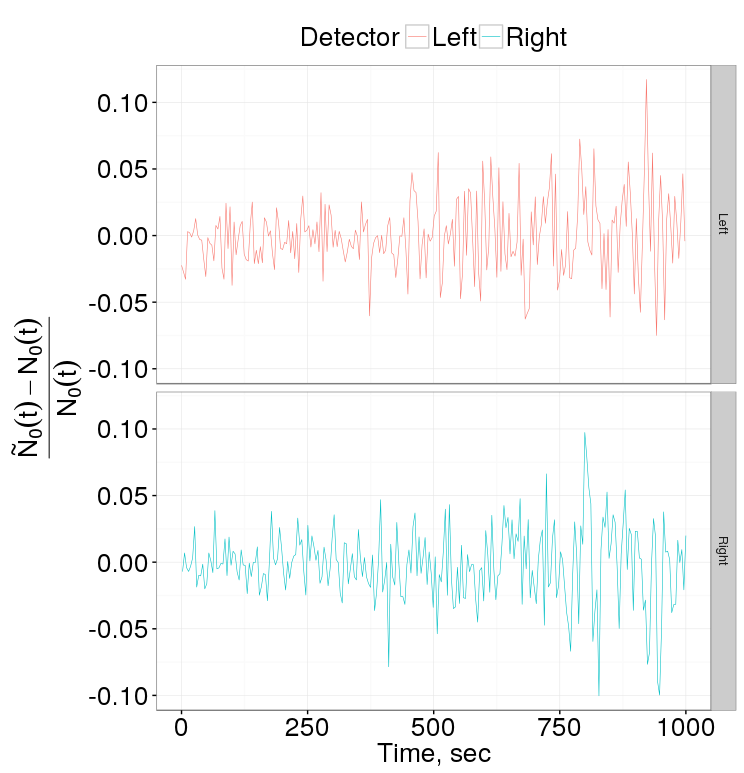
\includegraphics[width=.8\linewidth]{images/App_Stats/LR_detector_relErr}
	\caption{Относительная ошибка измерения частоты событий на правом и левом
		детекторах как функция времени.\label{fig:LRDetErr}}
\end{figure}

\begin{figure}[H]
	\centering
	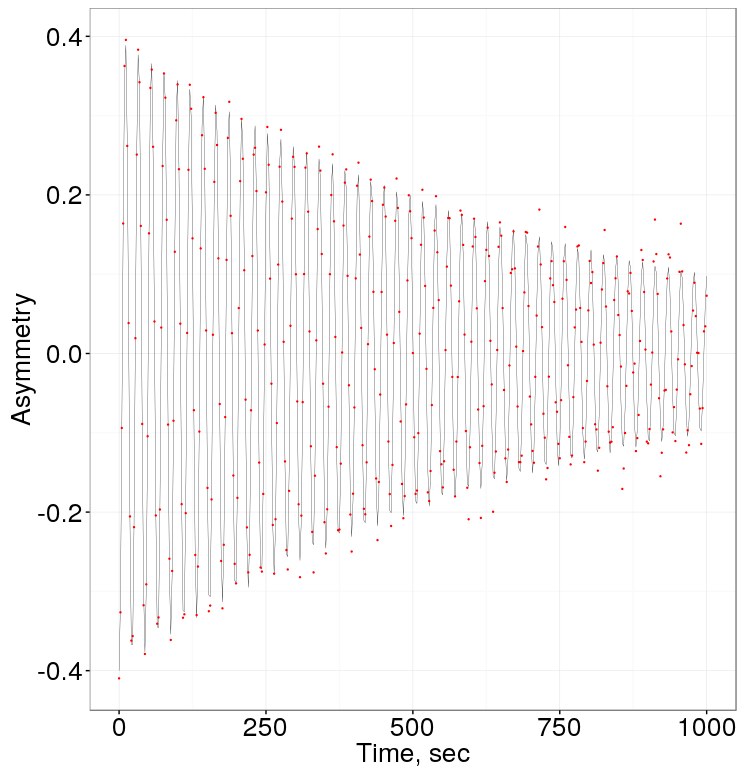
\includegraphics[width=.8\linewidth]{images/App_Stats/Asymmetry}
	\caption{Ожидание (чёрная линия) и измерения (красные точки)
		асимметрии сечения.\label{fig:Asym}}
\end{figure}

Если начальная оценка частоты, полученная из равномерной выборки, 
имеет стандартную ошибку порядка $10^{-6}$ рад/сек, симуляции
подтверждают, что при применении модулированной схемы выборки, 
стандартная ошибка оценки может быть улучшена до примерно $\vp{5.8}{-7}$ рад/сек, 
без учёта потери анализирующей способности детектора
при приближении вертикальной компоненты поляризации к нулю.



\end{document}
